\documentclass[fleqn,10pt,numbers]{olplainarticle}
\usepackage{float}
\usepackage{gensymb}
\usepackage{rotating}
\usepackage{booktabs}
\usepackage{graphicx}
\usepackage[labelfont=bf]{caption}
\usepackage{subcaption}
\usepackage{xr}
\externaldocument[si-]{supp_altstat}
\usepackage{hyperref}
\usepackage{xcolor}
\usepackage{todonotes}
% Arabic script for the one-time introduction of the Rub' al-Khali (pdflatex).
% arabtex redefines \begin so that every environment, including document,
% opens a group; restore LaTeX's \begin/\end after loading it.
\let\LaTeXbegin\begin \let\LaTeXend\end
\usepackage{arabtex}
\usepackage{utf8}
\setcode{utf8}
\let\begin\LaTeXbegin \let\end\LaTeXend
\hypersetup{hidelinks}

\title{Microbial biogeography and functional differentiation across the Rub' al-Khali}

\author[1,2]{Rund Tawfiq}
\author[1]{Marwa Abdelhakim}
\author[3]{Sulaiman M. Alajel}
\author[1]{Mohammed Alarawi}
\author[8]{Hind Aldakhil}
\author[1]{Abderahmane Derouiche}
\author[5]{Daniela I. Drautz-Moses}
\author[4]{Michel Dumontier}
\author[7]{Raik Grünberg}
\author[1]{Alejandra Lopez-Velazquez}
\author[9]{Susana Martinez Arbas}
\author[1]{Kexin Niu}
\author[1]{Krishnakumar Sivakumar}
\author[6]{Tiannyu Wang}
\author[5]{Xiang Zhao}
\author[1]{Jood Zubair}
\author[6]{Magnus Rueping}
\author[1]{Robert Hoehndorf\thanks{Correspondence:
  robert.hoehndorf@kaust.edu.sa}}
%% ORCIDs received from co-authors (August 2026), for the submission system;
%% the olplainarticle class has no ORCID field.
%%   Daniela I. Drautz-Moses    0000-0002-3739-0917
%%   Susana Martinez Arbas      0000-0001-7309-8190
%%   Alejandra Lopez-Velazquez  0009-0001-2873-5311
%%   Xiang Zhao                 0009-0007-8662-9406
%%   Jood Zubair                0009-0005-9532-0801
%%   Abderahmane Derouiche      0000-0002-3241-1424
%%   Kexin Niu                  0000-0002-7302-0462
%%   Hind Aldakhil              0000-0001-9491-103X
%%   Mohammed Alarawi           0000-0001-8986-8209
%%   Rund Tawfiq                0000-0002-7052-573X  (ORCID registry, 6 Sep; to confirm)
%%   Marwa Abdelhakim           0000-0001-6816-2119  (ORCID registry, 6 Sep; to confirm)
%%   Michel Dumontier           0000-0003-4727-9435
%%   Raik Grünberg              0000-0001-9532-6043
%%   Robert Hoehndorf           0000-0001-8149-5890

\affil[1]{Bio-Ontology Research Group (BORG), Computer, Electrical and
  Mathematical Sciences and Engineering (CEMSE) Division, King Abdullah
  University of Science and Technology (KAUST), Thuwal, Saudi Arabia}
\affil[2]{Sano Centre for Computational Personalised Medicine, Krak\'{o}w, Poland}
\affil[9]{NIUM, Esch-sur-Alzette, Luxembourg}
\affil[3]{Ministry of Environment, Water and Agriculture, Saudi Arabia}
\affil[4]{Institute of Data Science, Department of Advanced Computing
  Sciences, Faculty of Science and Engineering, Maastricht University,
  Maastricht, The Netherlands}
\affil[5]{Bioscience Core Lab, King Abdullah University of Science and
  Technology, Thuwal, Saudi Arabia}
\affil[6]{Physical Science and Engineering (PSE) Division, King Abdullah
  University of Science and Technology (KAUST), Thuwal, Saudi Arabia}
\affil[7]{Biomedical Sciences Division (BioMed), King Abdullah University of Science and Technology (KAUST),
  Thuwal, Saudi Arabia}
\affil[8]{National Livestock \& Fisheries Development Program (NLFDP),
  Ministry of Environment, Water and Agriculture (MEWA), Riyadh 13413,
  Saudi Arabia}

\keywords{Rub' al-Khali, Empty Quarter, hyperarid soil microbiome, microbial
  biogeography, metagenome-assembled genomes, functional traits, trace-gas
  oxidation, $16$S rRNA amplicon survey}

\begin{abstract}
The Rub' al-Khali (Empty Quarter) is the world's largest continuous sand desert, but its soil microbial communities remain poorly characterised across the landscape and over repeated visits. We sampled 60 sites along a west--east transect of more than 1,000~km in five campaigns over 31 months, combining 1,186 16S rRNA gene profiles with genome-resolved metagenomics and environmental observations. Community dissimilarity increased with geographic distance, mainly through replacement of genera. The strongest change occurred in the eastern megabarchan field, where bacterial richness was 79\% lower than in the western uruq field and halotolerant genera were relatively enriched. MAG-based community profiles supported this eastern diversity decline. Within sites, root-adjacent soil had lower bacterial diversity and a distinct community compared with bulk soil. Genome-derived capacities connected these habitat differences to particular persistence strategies. Surface communities had greater representation of betaine-uptake and peroxide-defence genes, whereas root-adjacent communities showed selective depletion of group 1l hydrogenase genes; both shifts tracked community replacement under the analytical and foundational taxonomy snapshots. Other stress-response markers had heterogeneous or annotation-dependent contrasts. Spatial models and sampling-design simulations distinguished supported habitat associations from environmental gradients that the transect could not resolve. Together, these results connect microbial biogeography across the Empty Quarter to differences in encoded capacities for nutrient acquisition and stress protection.
\end{abstract}

\begin{document}

\flushbottom
\maketitle
\thispagestyle{empty}
\clearpage

\section*{Introduction}

Drylands are among the most extensive terrestrial biomes \cite{marasco2023diamonds}, and aridity is projected to increase across much of them \cite{maestre2015increasing}. Where plants are sparse and rainfall is rare, soil microbial communities carry much of the remaining biological activity \cite{makhalanyane2015microbial}. Soil microbes influence soil fertility and crop production, and drive environmental processes such as carbon and nitrogen fixation, organic matter decomposition, and greenhouse gas emissions \cite{ling2022rhizosphere,delgadobaquerizo2018global}. Bacteria isolated from dryland soils have been used to improve plant tolerance to abiotic stress \cite{eida2018desertplants} and to stabilize and restore degraded soils \cite{marasco2023diamonds}. Therefore, characterizing the composition and diversity of dryland soil microbiomes is relevant to agriculture, conservation, and land management.


The Rub' al-Khali (Arabic \RL{الربع الخالي}; in English, the Empty Quarter) is the world's largest continuous sand desert. It covers much of the southern Arabian Peninsula, mainly within Saudi Arabia, and is one of the least explored drylands in the world \cite{edgell2006arabian}. It is a hyperarid desert where rainfall is rare and temperatures approach $50\,^{\circ}\mathrm{C}$, making it one of the most extreme terrestrial environments on Earth \cite{crassard2013mundafan}. It is characterized by sand dunes and saline pans referred to as \textit{sabkhah}, and sparse shrubs and fauna \cite{mandaville_1986}. Ancient lakebeds are found throughout the desert, although it has no present link to rivers or other large water bodies \cite{edgell2006arabian}. Across this sand sea, steep transitions in dune morphology, evaporite mineral content, and sparse vegetation create distinct edaphic habitats under shared hyperarid climatic extremes \cite{edgell2006arabian,mandaville_1986}.


Desert soils have been studied at different scales. At large spatial scales, community composition differs between regions and along aridity gradients \cite{neilson2017significant}. In the Mojave desert, biological soil crust communities from central and southern sites had distinct compositions \cite{pombubpa2020mojave}. In the Atacama and Gobi deserts, the colonization and diversity of hypolithic communities declined as aridity increased \cite{warren2006hypolithic, wu2023seasonal}. Community composition also varied between habitats within a landscape, such as in the Namib desert, where a comparison of sand dune zones showed that each zone harbored a different bacterial community \cite{ronca2015namib}. At a smaller scale, some studies have shown that communities differed between surface and deeper soils. Surface and subsurface communities were distinct in Mojave soil crusts \cite{pombubpa2020mojave}, and microbial biomass in an Atacama playa decreased with depth \cite{horstmann2024atacama}. Also within sites, microbial communities differed between bulk soil and plant-associated soil, where the rhizosheath held more diverse communities than surrounding bulk soil in the Namib desert \cite{marasco2022namib}.


These spatial patterns have also been studied in relation to soil properties and environmental conditions. The distinct microbial communities in the Namib sand dunes varied with habitat stability, soil texture, and mineral and nutrient content \cite{ronca2015namib}. Decline in biomass with the depth gradient in the Atacama was linked to an increase in soluble salts \cite{horstmann2024atacama}. The Namib rhizosheath was found to be cooler, more humid, and richer in nutrients than bulk soil \cite{marasco2022namib}.


Desert soils have also been studied over time. Rainfall in deserts is rare, usually in short pulses, and the pulse--reserve model proposes that each pulse triggers a brief period of biological activity before the soil dries again \cite{noymeir1973desert, schwinning2004pulse}. In the Atacama desert, heavy rainfall re-distributed salts in the soil, and shifted community composition to be more similar to less arid sites \cite{uritskiy2019atacama,shen2021atacama}. Temperature has also been found to affect communities over time, where hypolithic communities in the Gobi desert were found to significantly differ from those sampled after cold periods \cite{wu2023seasonal}.


Studies that combine repeated sampling and large spatial scales in desert soils remain sparse \cite{yuan2017experimental}, and the Arabian Peninsula remains underrepresented in global studies \cite{maestre2015increasing, blancosacristan2025biocrust}. In the Arabian Peninsula, studies have described microbial communities along elevation gradients \cite{yasir2015elevation}, at single locations \cite{khan2020saudi}, in plant-associated soil \cite{osman2016jizan,eida2018desertplants,jalal2022saudi}, and in an inland sabkha of the Empty Quarter in the United Arab Emirates \cite{mckay2016sabkha}.

The Empty Quarter has not yet been surveyed across its landscape or over repeated visits, leaving unresolved how taxonomic turnover across dune fields and soil compartments relates to the genomic capacities that support persistence under hyperarid conditions \cite{ji2017atmospheric,cordero2019atmospheric,bay2021trace,bay2021aridity,ayalaortiz2025arid}. Here, we surveyed microbial communities at 60 sites along a 1,043~km west--east transect through the Saudi Empty Quarter in five campaigns over 31 months, sampling surface, shallow-subsurface and root-adjacent soil. We combined 1,186 16S rRNA gene profiles with soil pH, X-ray fluorescence elemental composition and climate summaries, and integrated these data with 546 core-transect shotgun metagenomes and 5,438 species-representative metagenome-assembled genomes (MAGs) curated in a companion data resource \cite{rubalkhali_datapaper}. Using hierarchical spatial models and simulations on our sampling design to distinguish supported habitat associations from collinear regional gradients, we tested whether community differentiation across dune fields and soil compartments occurs primarily through lineage replacement and whether this replacement reorganises encoded capacities for compatible-solute acquisition, oxidative and photoprotective defence, and high-affinity atmospheric trace-gas oxidation. All analysis inputs and code are available in \href{https://github.com/bio-ontology-research-group/empty-quarter-ecology}{the ecology reproducibility repository}.

\section*{Results}\label{sec2}

\subsection*{Environmental and taxonomic gradients across the Rub' al-Khali}
We surveyed 60 sites along a west--east transect through the Empty Quarter in Saudi Arabia in five campaigns over 31 months (Figure~\ref{fig:landscape}a). Western sites were characterized by uruq dunes and rocky outcrops, central sites by pale linear dunes, and eastern sites by large red megabarchans interspersed with inland saline pans known as \textit{sabkhas} (Figure~\ref{fig:landscape}b--e). Field observations classified 44 sites as sand dunes, nine as saline pans, three as oases and four as other landforms (Supplementary Figure~\ref{si-fig:landforms}).

\begin{figure}[!htbp]
\centering
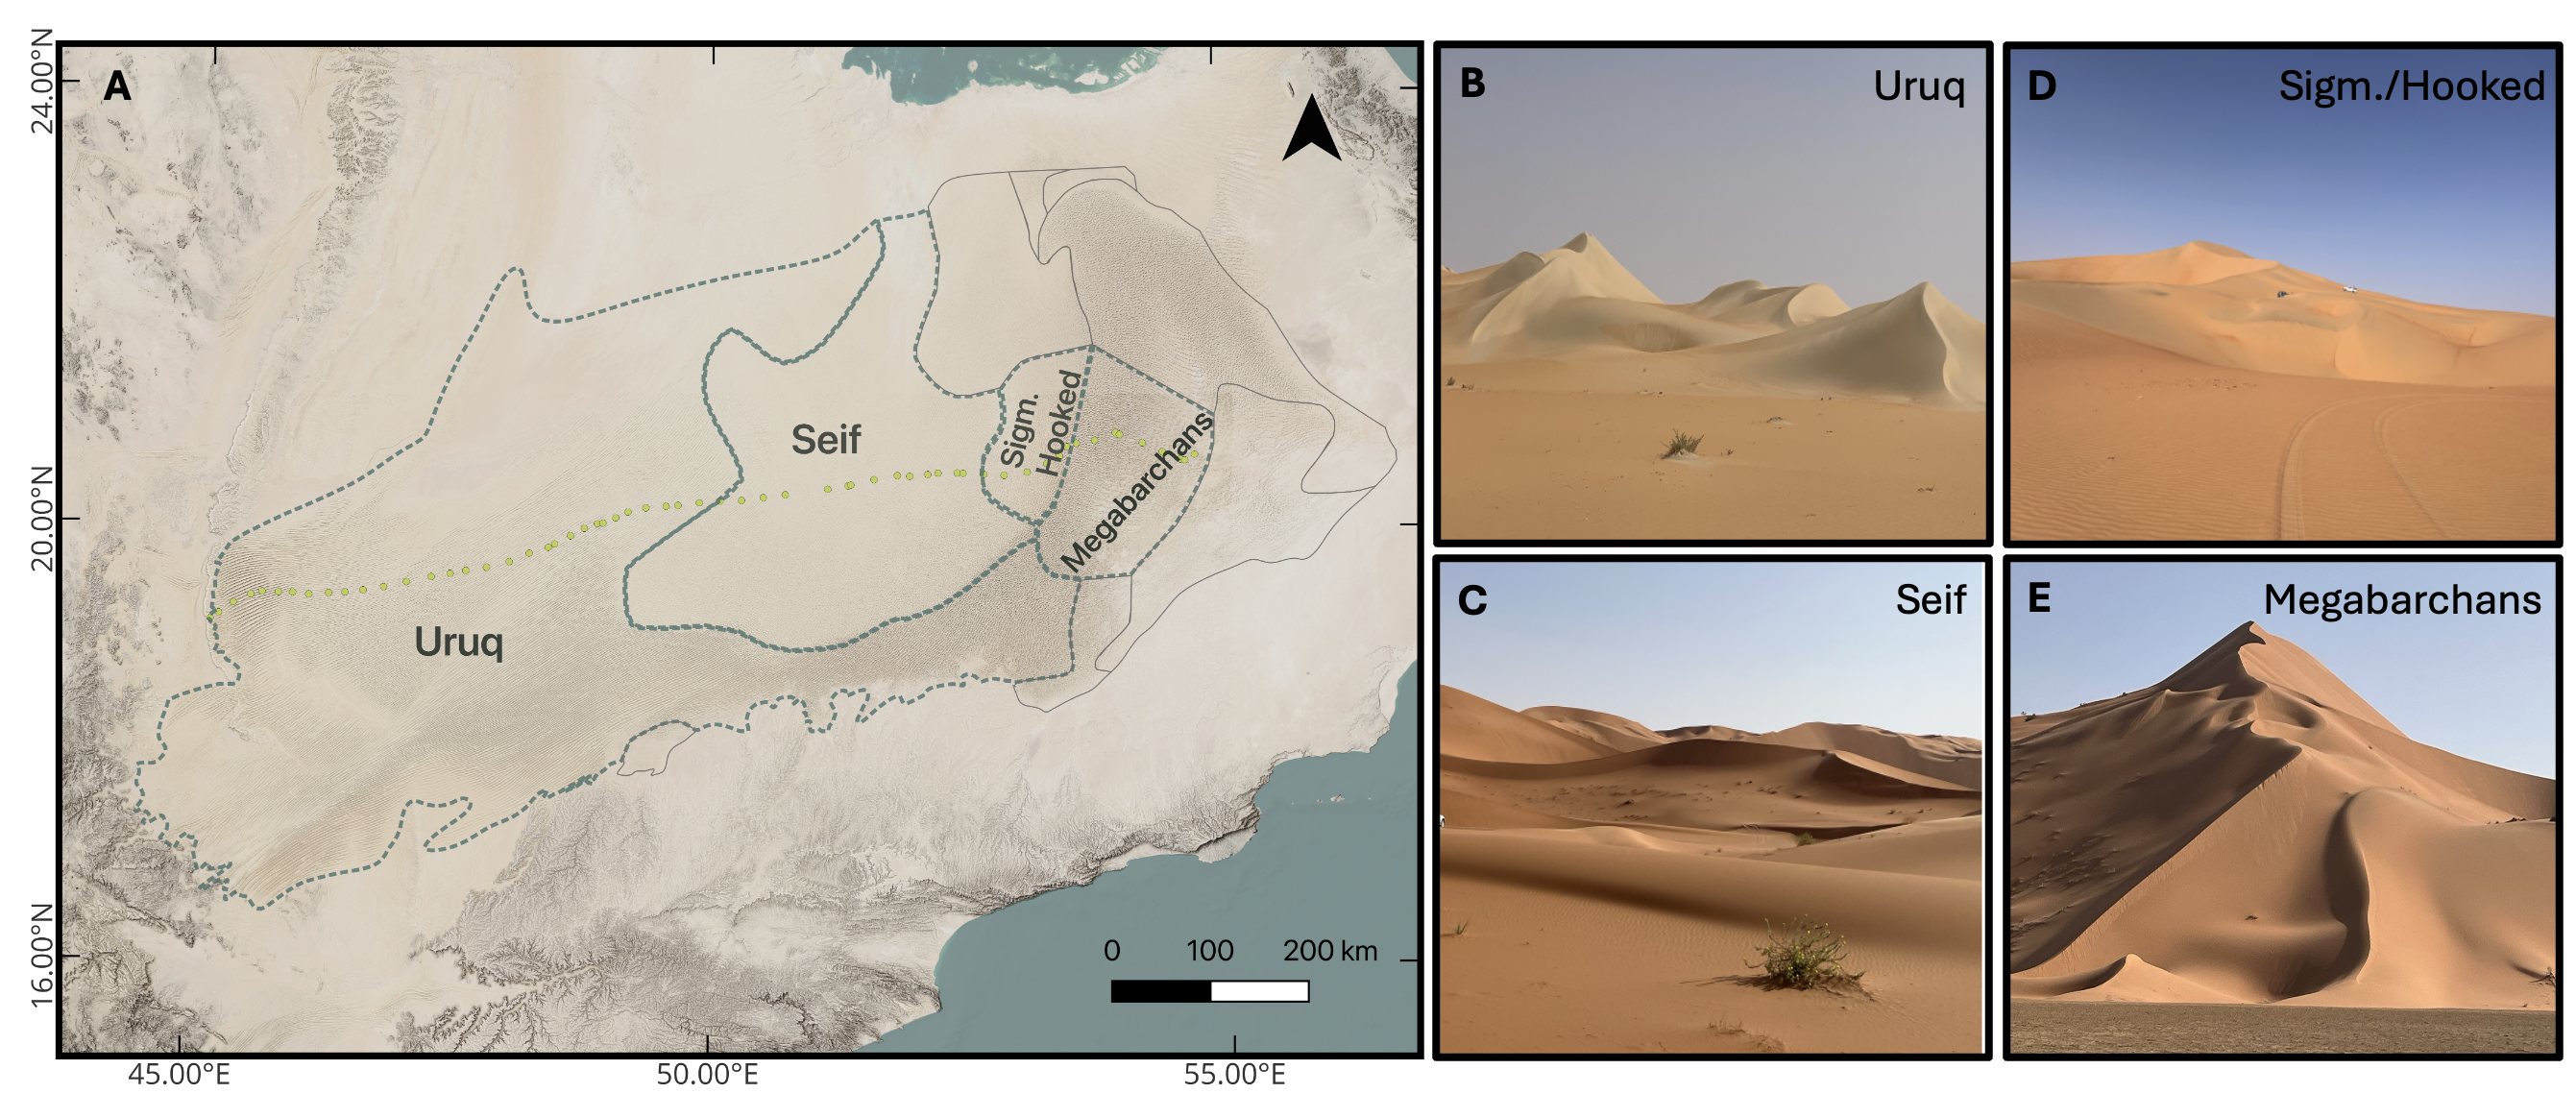
\includegraphics[width=\linewidth]{updated_figures/fig_landscape.png}
\caption{Study area. (A) Sampling sites along the transect and dune subtypes on an Esri Terrain basemap. Examples of dunes across the transect showing uruq (B), seif (C), sigmoidal and hooked (D), and megabarchan (E) dunes.}
\label{fig:landscape}
\end{figure}

Climate and soil chemistry varied along the same geographic gradient (Figure~\ref{fig:phyla_landscape}b,c). Mean air temperature over the 49-month observation period increased from $26.4\,^{\circ}\mathrm{C}$ in the west to $30.3\,^{\circ}\mathrm{C}$ in the east, while relative humidity increased from $24.3\%$ to $35.4\%$ (Supplementary Figure~\ref{si-fig:climate_samples}a). Both were strongly correlated with transect position ($r = 0.93$ and $0.92$, respectively). Site mean soil pH increased from $7.7$ to $8.5$ ($r = 0.84$). The first principal component (PC1) of soil X-ray fluorescence (XRF) measurements explained $39.2\%$ of elemental variance. The elemental score loaded mainly on Ca, Mg, Na, S and Cl, and negatively on Si (Supplementary Table~\ref{si-tab:xrf_elements}), consistent with a shift from quartz-rich sand towards soils richer in carbonate and evaporite minerals \cite{mckay2016sabkha,eggleston2020hydrogeologic}. It increased eastward but was less closely related to transect position ($r = 0.68$) than pH or climate, mainly due to variation between sites in the eastern dune fields.
%Element-level patterns are given in Supplementary Section~\ref{X}.

Across 1,186 samples from the 16S rRNA gene catalogue (Supplementary Figure~\ref{si-fig:climate_samples}b) bacterial communities were dominated by Pseudomonadota, Bacillota and Actinomycetota (Figure~\ref{fig:phyla_landscape}a). Acidobacteriota and Verrucomicrobiota, which are among the most abundant phyla in global soil surveys \cite{delgadobaquerizo2018global,fierer2017embracing}, together accounted for $3.2\,\%$ of reads. Phylum composition changed from west to east, where Bacillota increased from $19\,\%$ of reads in the uruq dune field to $35\,\%$ in the megabarchan field, whereas Actinomycetota decreased from $22$ to $9\,\%$ and Chloroflexota from $10$ to $4\,\%$. At the genus level, \textit{Domibacillus} ($6.1\,\%$) was the most abundant genus in every compartment, followed by \textit{Massilia} ($3.4\,\%$), \textit{Bacillus} ($3.3\,\%$), \textit{Microvirga} ($2.4\,\%$) and \textit{Flavisolibacter} ($2.0\,\%$). ASVs without a genus assignment made up $35.5\,\%$ of reads per sample on average.

\todo[inline]{add a paragraph}



\begin{figure}[!htbp]
\centering
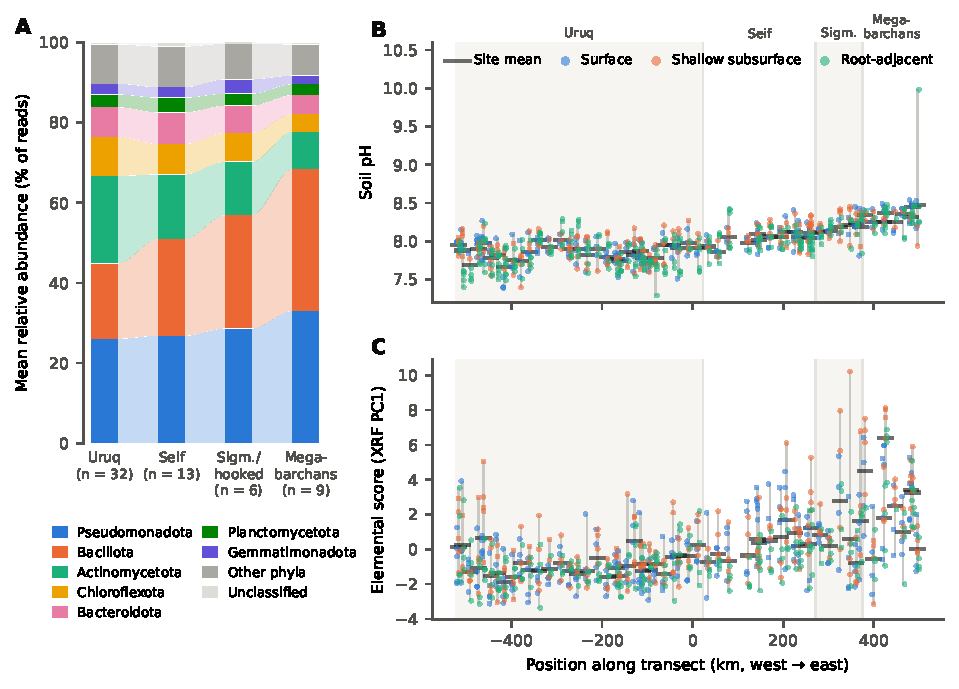
\includegraphics[width=\linewidth]{updated_figures/fig_phylum_ph_xrf.pdf}
\caption{Phylum composition and soil physiochemical properties by dune subtype. (A) Relative abundances of soil bacterial community at the phylum level compared across the dune zones. Soil pH (B) and elemental score (C) variation by compartment and dune zone along the transect.}
\label{fig:phyla_landscape}
\end{figure}

\begin{figure}[!htbp]
\centering
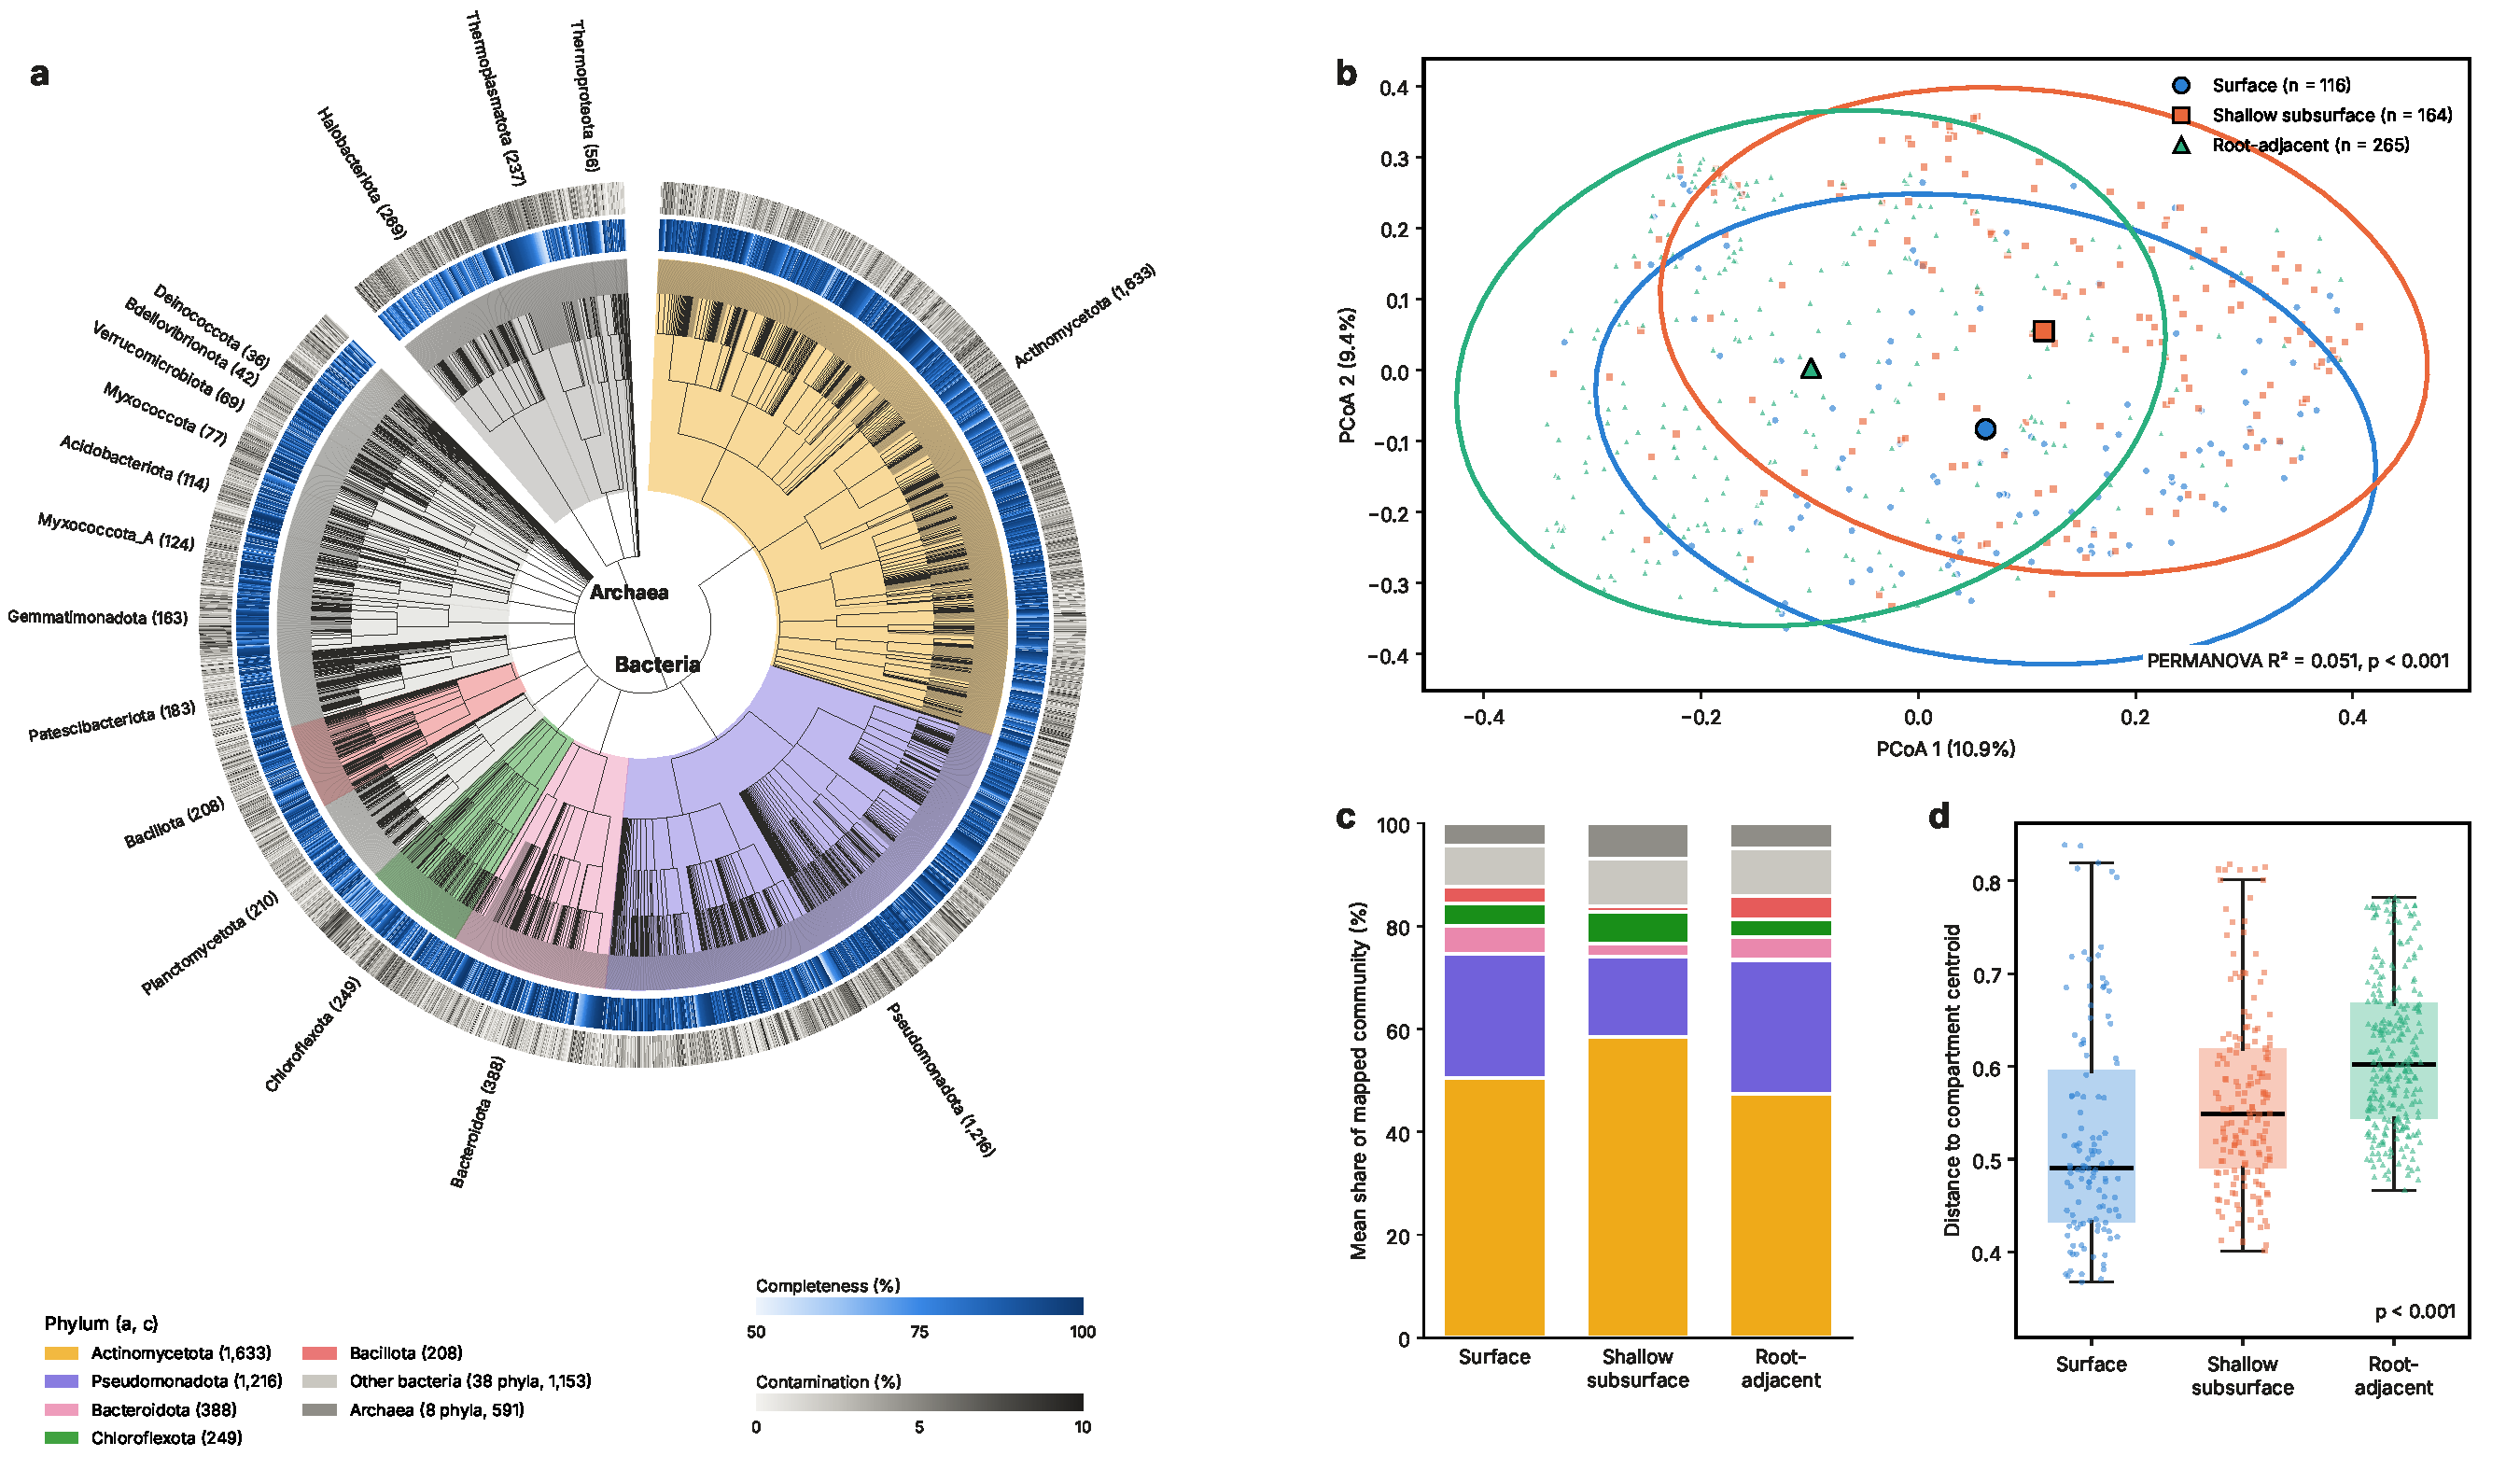
\includegraphics[width=\linewidth]{updated_figures/figure1_mags.pdf}
\caption{(a) Phylogenetic tree of the $5,438$ species representatives from the MAGs according to their GTDB assignment, and completeness and contamination from CheckM. (b) Principal coordinate analysis (PCoA) of MAG composition across compartments. (c) Mean share of mapped reads for each phylum across compartments. (d) Dispersion (median distance from compartment centroid) across compartments.}
\label{fig:mag_landscape}
\end{figure}
\todo[inline]{Change to actual phylogenetic tree w/ distances}
%%%%%%%%%%%%%%%
\subsection*{Community composition turns over gradually across the desert}

Bacterial communities became more dissimilar with geographic distance (Supplementary Table~\ref{si-tab:decay}, Figure~\ref{fig:distancedecay}a). Aitchison distance increased with geographic distance in all compartments (surface: $1.35$ per 100~km, 95\% CI $0.48$, $2.22$; shallow subsurface: $1.51$, 95\% CI $0.54$, $2.47$; root-adjacent soil: $1.18$, 95\% CI $0.20$, $2.15$). Decay appeared steeper in shallow subsurface than in root-adjacent soil (+0.33 per 100 km, block-jackknife interval 0.07–0.60), but block-jackknife intervals for differences between compartments covered the true difference in only 77–81\% of simulations (Supplementary Section~\ref{si-decay_calibration}), so this difference is uncertain. Differences between surface soil and the other compartments were smaller (0.16--0.17) and their intervals included zero. Dissimilarity increased most rapidly over the first 250~km ($1.5$--$2.1$ Aitchison units per 100~km), with a progressively weaker increase at greater distances.
%Most dissimilar site pairs were not necessarily the farthest apart, as most involved at least one site in the megabarchan field (74–98\% of the 50 most dissimilar pairs per compartment).
% Uncertainty intervals were estimated using a jackknife that removed contiguous blocks of sites, which maintained nominal coverage in simulation.

Dune field accounted for additional differences in community composition beyond geographic distance. Including dune field reduced the distance decay slopes ($-$12--25\%), but geographic distance remained positively associated with Aitchison distance in all compartments (Supplementary Table~\ref{si-tab:decay_dune}). After accounting for geographic distance, each additional megabarchan site in a pair was associated with greater dissimilarity in shallow subsurface soil ($7.3$ Aitchison units, $95\,\%$ CI $0.5$--$14.1$) and root-adjacent soil ($6.9$, $95\,\%$ CI $1.0$--$12.9$). In surface soil, the megabarchan estimate was positive but uncertain ($5.0$, $95\,\%$ CI $-2.0$ to $12.1$), and pairs involving the sigmoidal and hooked dune field were more dissimilar ($2.4$, $95\,\%$ CI $0.9$--$4.0$). At equivalent distances, pairs from different dune fields were on average more dissimilar than pairs within a field ($3.9$--$4.3$ Aitchison units), but these differences were unsupported (intervals included zero). In a distance-matched comparison, the difference fell from $4.2$--$4.6$ to $1.4$--$2.5$ units when pairs involving megabarchan sites were excluded (Supplementary Table~\ref{si-tab:decay_dune}). Consistent with this finding, $74$--$98\,\%$ of the $50$ most dissimilar pairs in each compartment included at least one megabarchan site.

Mean S\o{}rensen dissimilarity was similar across compartments ($0.41$--$0.42$, SD $\pm0.10-0.15$ across site pairs), and turnover accounted for $71$--$76\,\%$ of dissimilarity (Supplementary Table~\ref{si-tab:decay}). Differences between sites therefore reflected mainly replacement of genera rather than nestedness, in which poorer sites hold subsets of the genera at richer sites. Sørensen dissimilarity increased with geographic distance in root-adjacent soil (slope = $0.017$, 95\% CI $0.002$, $0.032$), whereas no detectable relationship was found in surface or shallow subsurface soil after accounting for dependence between site pairs (intervals include zero; Supplementary Table~\ref{si-tab:decay}).

\begin{figure}[!htbp]
\centering
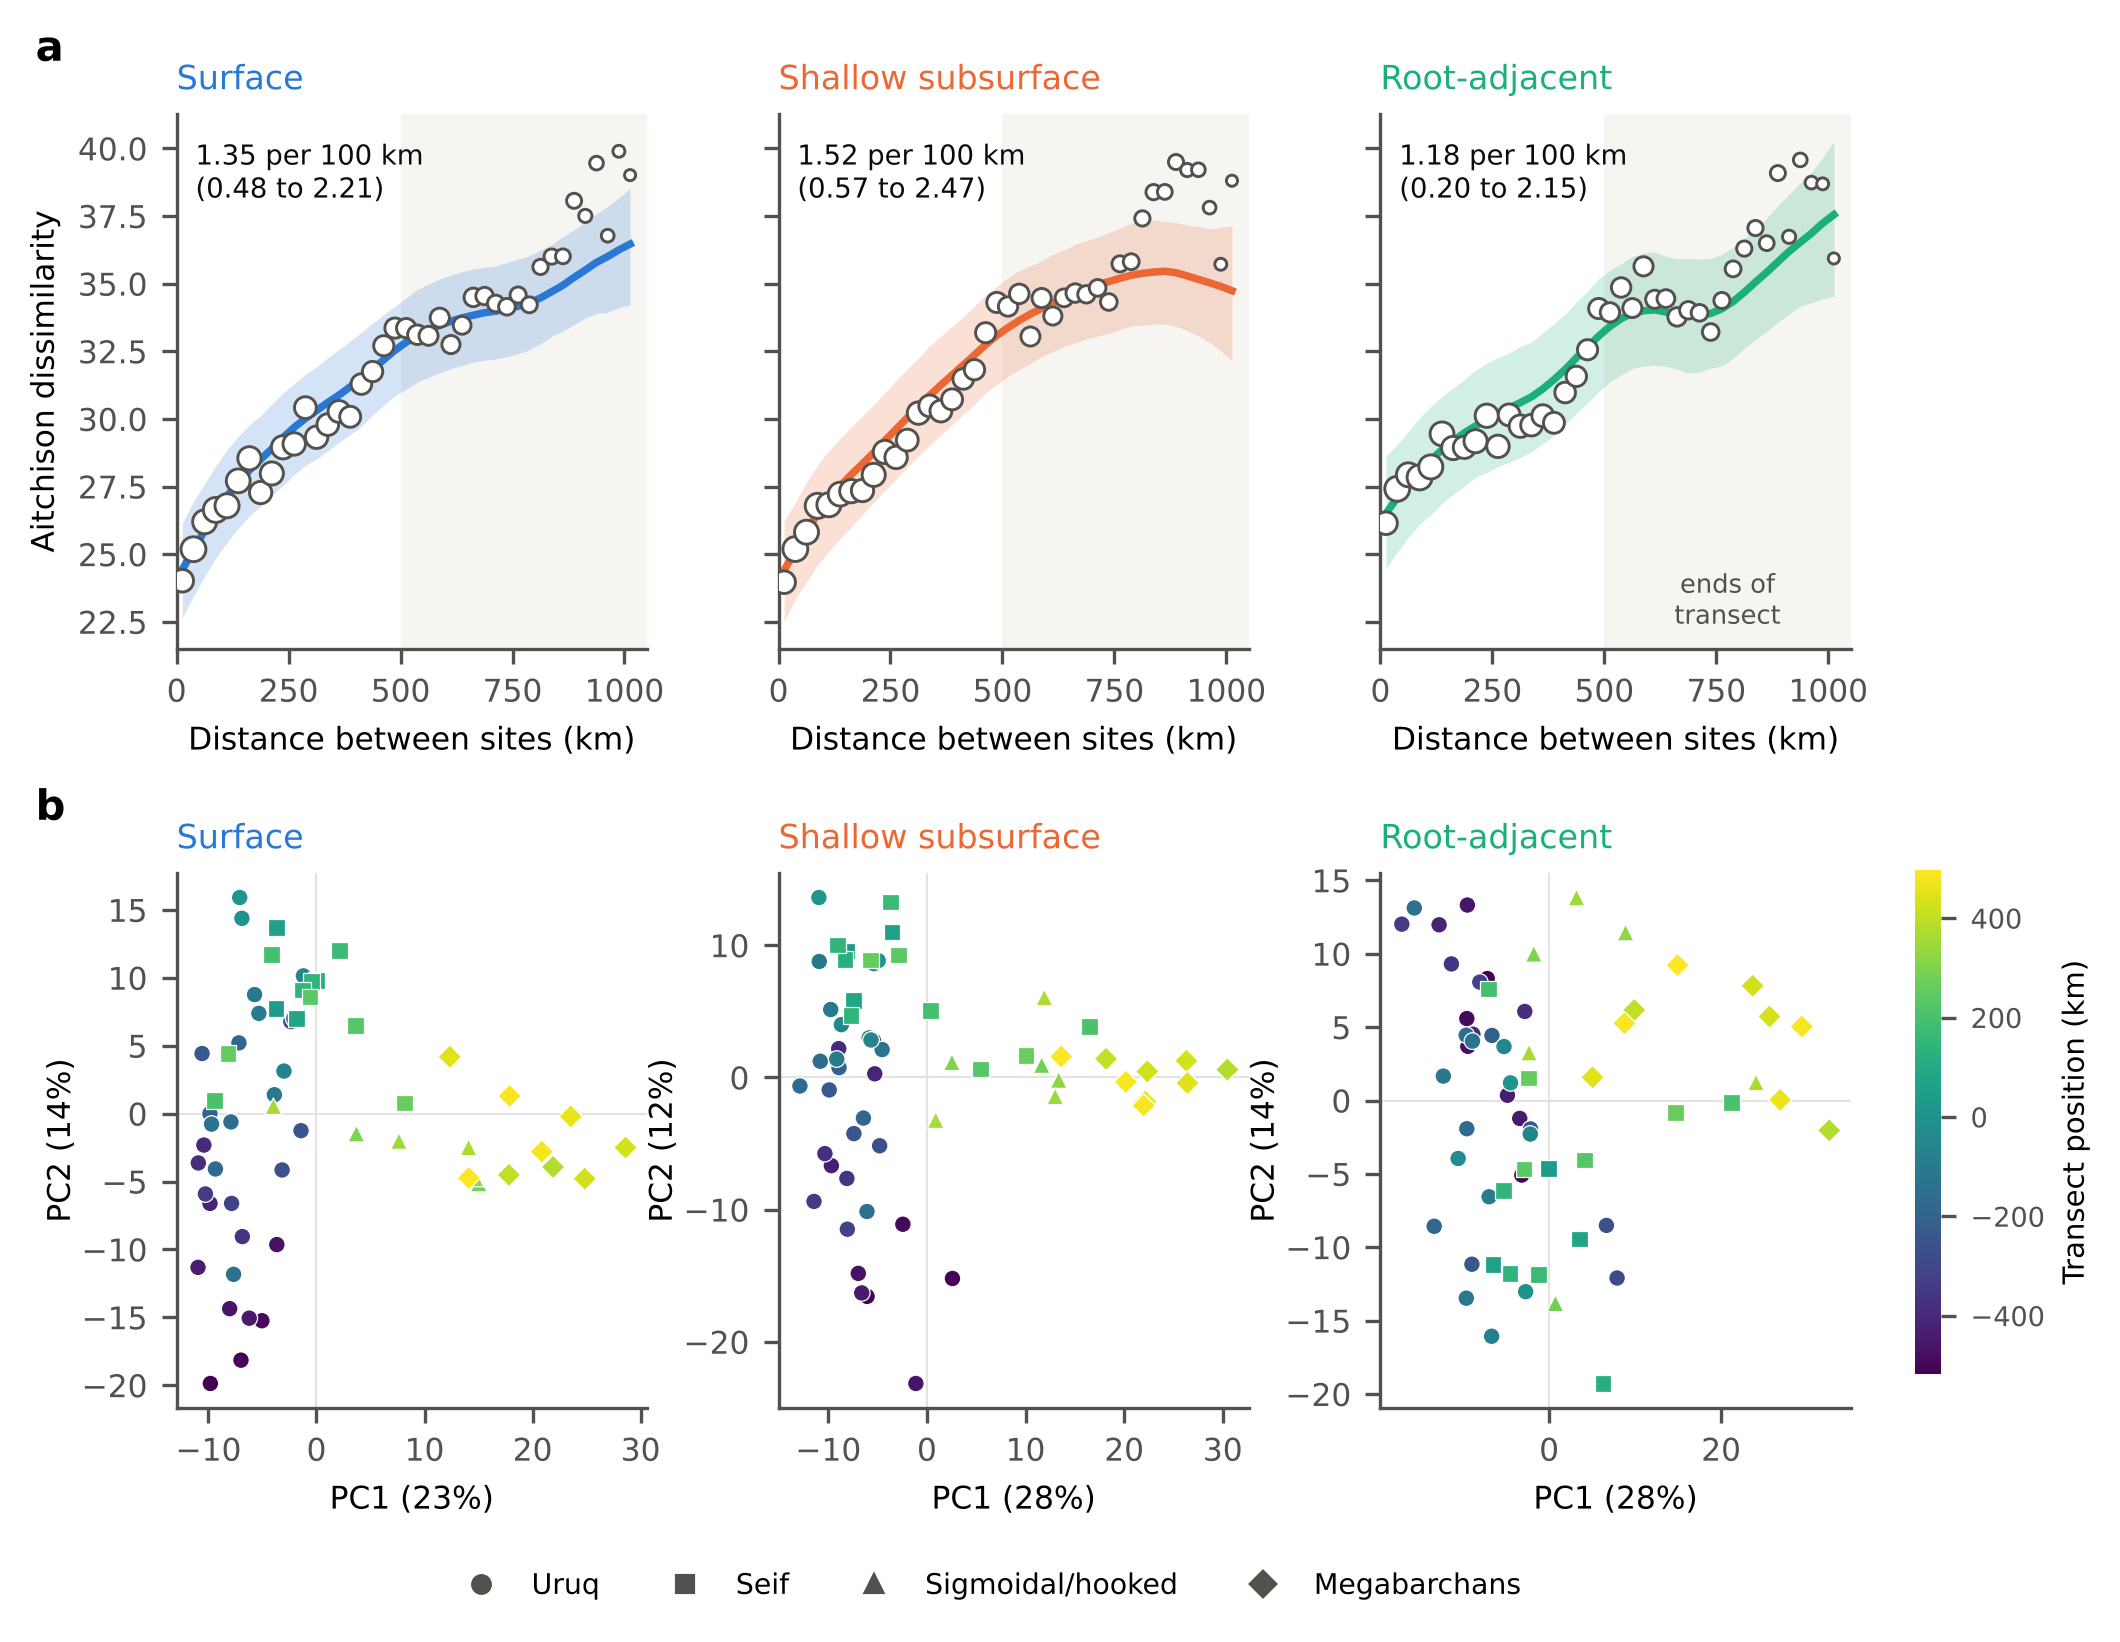
\includegraphics[width=\linewidth]{updated_figures/fig5_distance_decay.png}
\caption{Community composition over distance. (a) Aitchison distance between sites against geographic distance in each compartment. Points are mean dissimilarities sized by the number of site pairs. Lines and shaded bands show the median and $95\,\%$ credible interval. Values are the linear slope per $100$~km with its $95\,\%$ interval. Beyond $500$~km (grey), all pairs include sites near the two ends of the transect. (b) Principal component analysis (PCA) of site mean CLR profiles in each compartment.}
\label{fig:distancedecay}
\end{figure}

% \todo[inline]{move elsewhere}
% Differences in elemental score between sites were moderately correlated with geographic distance ((r = 0.40)), while differences in pH were more strongly correlated ((r = 0.67)). Nevertheless, greater differences in elemental score were associated with greater community dissimilarity in all three compartments, after accounting for geographic distance (2.3–3.4 Aitchison units per standard deviation of elemental difference). Including elemental differences reduced the estimated distance-decay slopes by 28–49\%, with the largest reduction in root-adjacent soil. However, these reductions were imprecisely estimated, with intervals including zero in all compartments. Differences in pH added no explanatory power after accounting for distance and elemental differences. These results suggest that variation in elemental chemistry is associated with some of the spatial variation in community composition, although its contribution to distance decay remains uncertain.

%%%%%%%%%%%%%%%

\subsection*{Diversity is stable across most of the Rub' al-Khali, and declines sharply in the east}

%Studies have shown that soil microbial diversity decreases with increasing temperature \cite{zhao2024effects}, and that diversity peaks near neutral pH \cite{lauber2009pyrosequencing}. We therefore expected alpha diversity to decline towards the eastern dunes with higher temperatures and more alkaline soils (Supplementary Figure~\ref{si-fig:climate_samples}a).
Alpha diversity was stable across most of the sampled transect and declined in the eastern dune fields (Figure~\ref{fig:alpha_transect}, Supplementary Table~\ref{si-tab:dune_alpha}). Richness and Shannon diversity were comparable between the uruq and seif fields (richness: $-7\%$, $95\%$ CrI $-23$ to $27\%$; Shannon: $-0.15$ nats, $95\%$ CrI $-0.43$ to $0.21$). In the sigmoidal and hooked dune field, richness was $44\%$ lower than in the uruq field ($95\%$ CrI $-56$ to $-15\%$), although the difference in Shannon diversity was less certain ($-0.52$ nats, $95\%$ CrI $-0.87$ to $0.01$). The strongest decline occurred in the megabarchan field, where richness was $79\%$ lower and Shannon diversity was $1.65$ nats lower than in the uruq field ($95\%$ CrIs $-84$ to $-68\%$ and $-2.03$ to $-1.13$, respectively). Normalized Shannon diversity was also lower in the megabarchan field ($-0.088$, $95\%$ CrI $-0.116$ to $-0.059$), indicating that the decline was not explained solely by lower richness but also involved a change in the distribution of abundances among genera.

%The very low-diversity profiles behind the eastern decline were retained after quality checks (Supplementary Section~X).

This pattern was more closely associated with dune field than with geographic position alone (Supplementary Table~\ref{si-tab:dune_cv}). Although richness was initially strongly spatially structured, accounting for dune field improved predictions of richness and both Shannon diversity measures (leave-site-out log score gains of $29.8$, $21.6$ and $11.4$, respectively). It also reduced the remaining spatial variation in richness (SD $\pm0.56$ to $\pm0.09$). The eastern decline therefore reflects a more step-wise decrease between dune fields rather than a gradual decline with distance along the transect.


%Between sites, higher soil elemental scores were associated with lower richness and Shannon diversity, independently of the spatial field (Supplementary Table~\ref{si-tab:between_site}). This association weakened when dune field was included and when the low diversity samples were excluded. Site mean pH was not clearly associated with diversity once the spatial field was included. Long-term humidity, but not temperature, followed the eastern decline. Both are almost exact functions of position along the transect, and simulation showed that their effects cannot be separated from spatial variation in this design (Supplementary Section~\ref{si-identifiability}). We therefore treat climate as a description of the gradient.



\begin{figure}[!htbp]
\centering
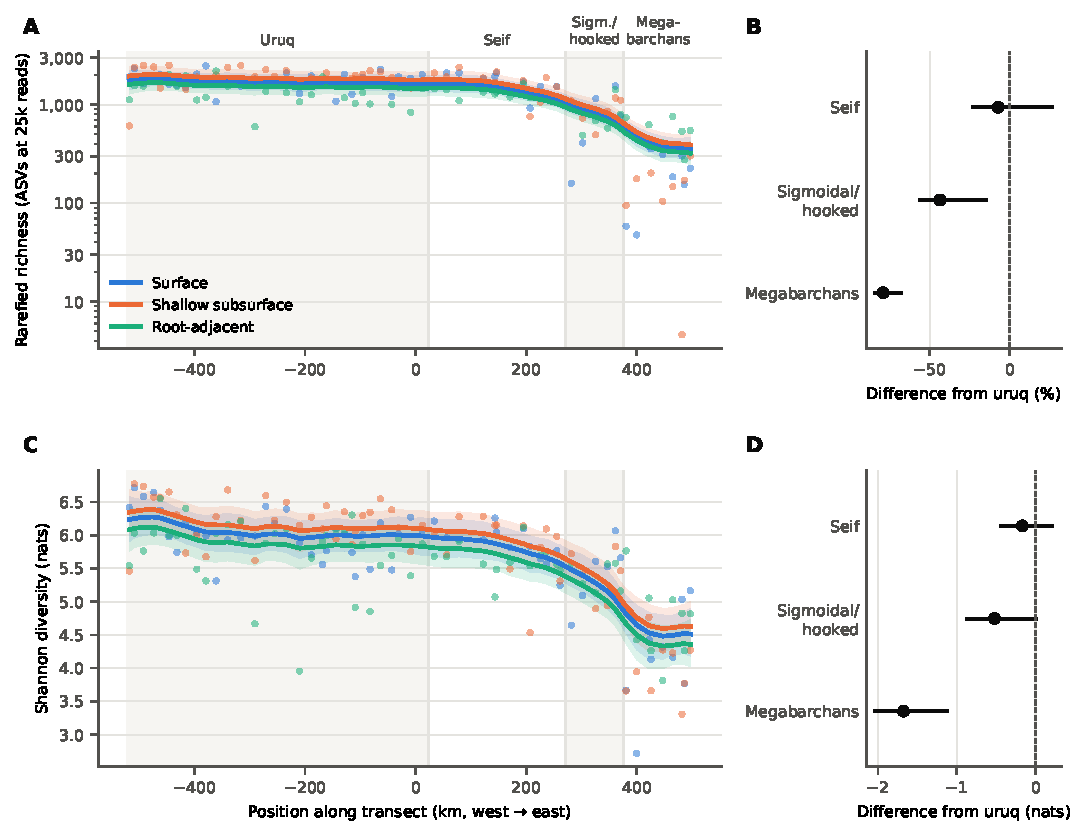
\includegraphics[width=\linewidth]{updated_figures/fig_alpha_transect.pdf}
\caption{Diversity across the transect and dune fields. (A, C) Rarefied ASV richness and Shannon diversity by transect position and soil compartment; curves describe the west--east pattern. (B, D) Estimated differences from the uruq field, with 95\% credible intervals from the spatial models. Richness contrasts are percentages and Shannon contrasts are in nats.}
\label{fig:alpha_transect}
\end{figure}

In models with dune field and the spatial field, the presence of 142 of the 200 genera and the abundance of 63 differed between the four dune fields (Wald tests, FDR 5\%; Figure~\ref{fig:genus_models}). Nearly all differences involved the megabarchan field, as no genus differed between the seif and uruq fields in abundance, and only 8 in presence, whereas 152 genera differed in presence and 51 in abundance between the megabarchan and uruq fields. Most of these genera were less often present in the megabarchan field (142 of 152), consistent with its lower richness. Relative to the average genus, 44 genera differed in presence and 55 in abundance in the megabarchan field. Genera of halotolerant Bacillota (\textit{Aquibacillus}, \textit{Sediminibacillus}, \textit{Halalkalibacter}) and \textit{Halomonas} were relatively enriched, whereas \textit{Aridibacter}, \textit{Nocardioides}, \textit{Rubrobacter} and \textit{Flavisolibacter} were depleted.

\begin{figure}[!htbp]
\centering
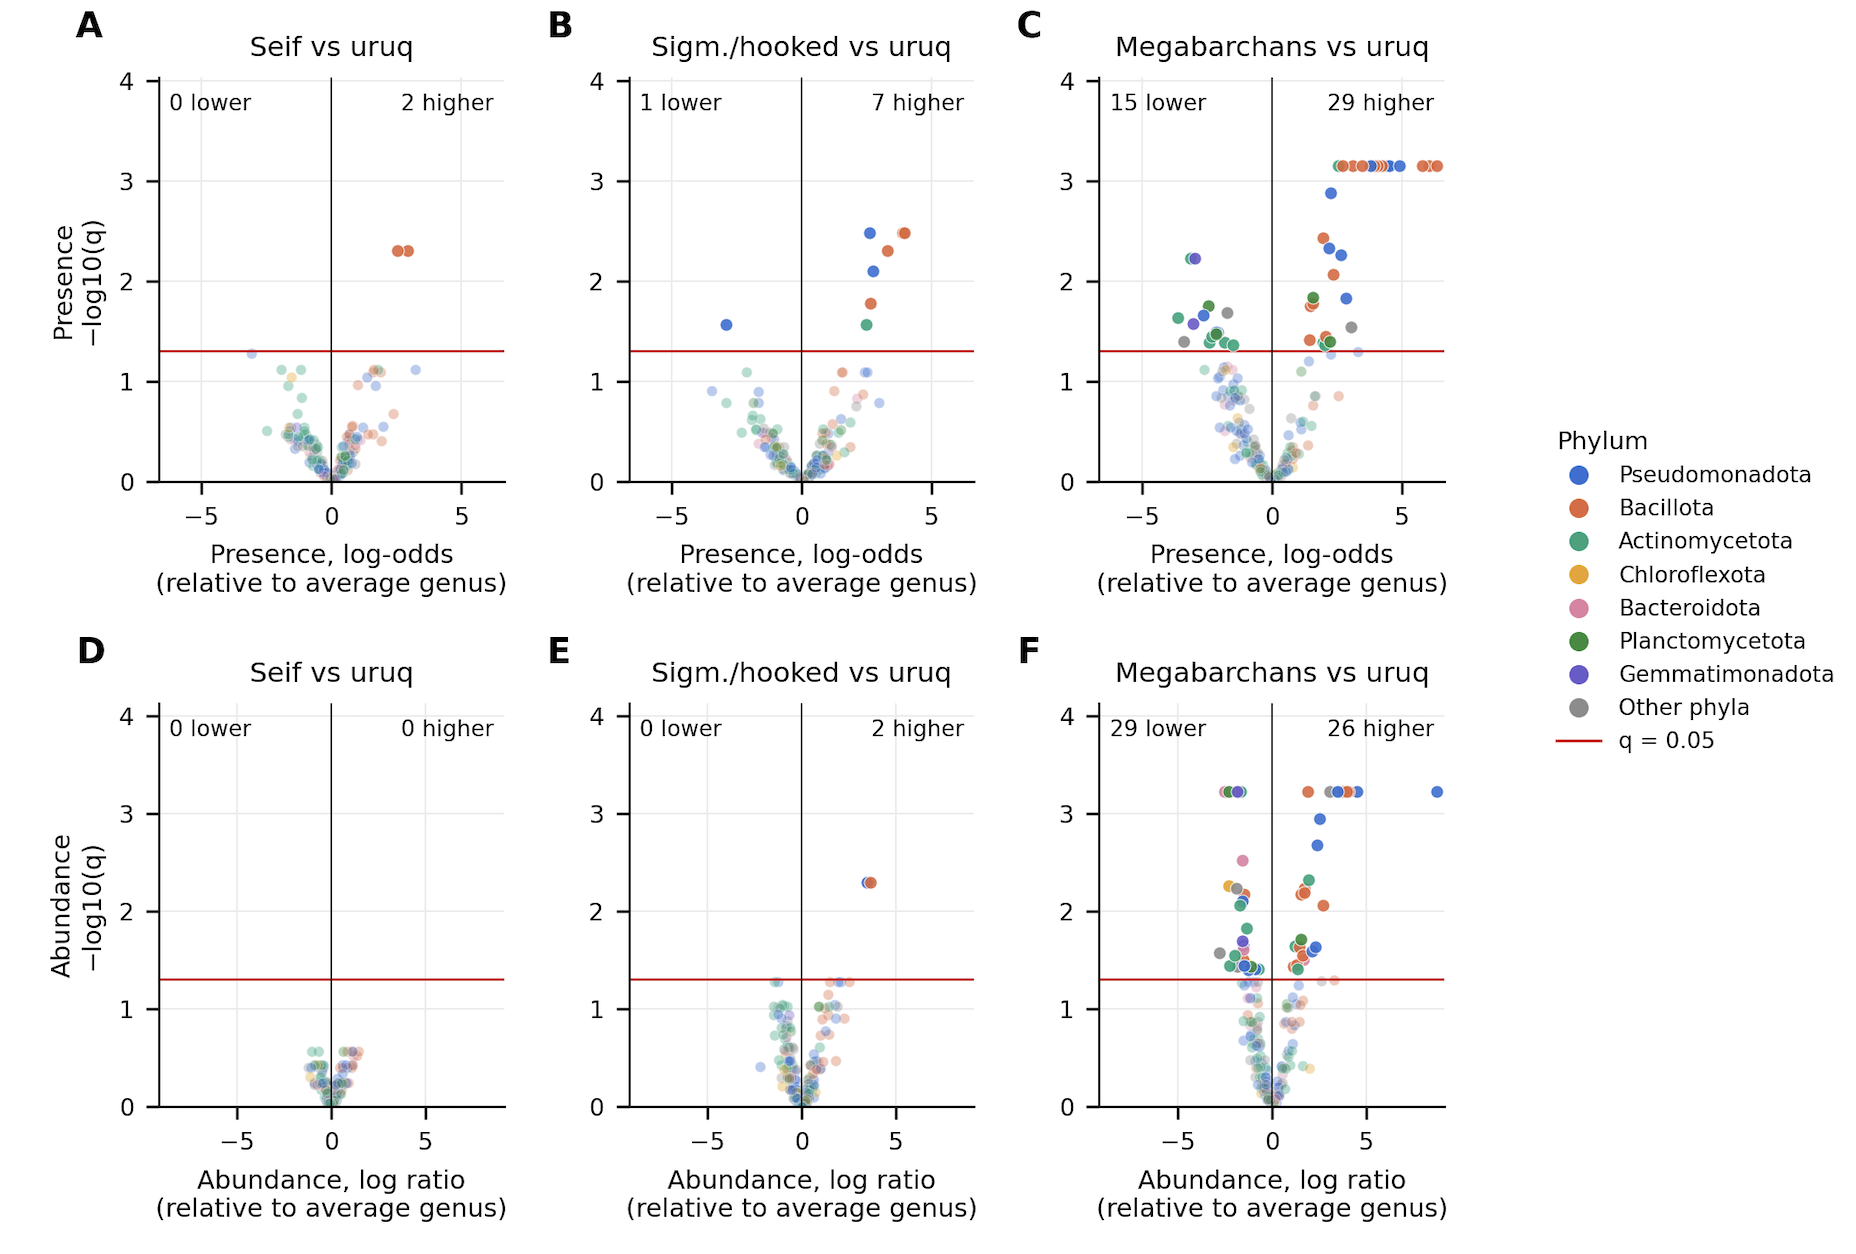
\includegraphics[width=\linewidth]{updated_figures/Genus_models.png}
\caption{Genus differences between dune fields. Volcano plots of the presence (\textbf{A}--\textbf{C}, log-odds) and abundance where present (\textbf{D}--\textbf{F}, log ratio) of the 200 most abundant genera in each dune field relative to the uruq field, from hurdle models with dune field and the spatial field. Effects are relative to the average genus. Points are genera, colored by phylum. Red line marks $q = 0.05$. Values of $q$ are bounded below by the 20,000 posterior draws.}
\label{fig:genus_models}
\end{figure}

Shotgun metagenomic profiles from 546 samples mapped against the 5,438 species representative genomes supported this eastern taxonomic decline. In spatial models across the metagenomes adjusting for campaign, read depth and soil compartment, bacterial MAG Hill diversity ($q=1$) was lower in the eastern megabarchan field than in the western uruq field ($-1.132$ log units, 95\% CrI $-1.589$ to $-0.327$; $68\%$ lower effective genome diversity), and the contrast persisted in the 441-library matched amplicon--metagenome model cohort ($-1.224$ log units, 95\% CrI $-1.694$ to $-0.471$; Supplementary Table~\ref{si-tab:mag_spatial}). By contrast, annotated KEGG Orthology (KO) copy number Hill diversity ($q=1$) across the same metagenomes showed little difference in the megabarchan field ($+0.025$ log units, 95\% CrI $-0.022$ to $0.073$; conditional joint spatial-block sensitivity in Supplementary Table~\ref{si-tab:stage4_joint_diversity}). Thus the strong eastern decline in bacterial genome diversity was not accompanied by a similarly large decline in this summary of annotated KO diversity.

%%%%%%%%%%%%%%%

\subsection*{Soil elemental score is weakly associated with diversity, whereas pH shows no clear association}
%Studies have shown that soil microbial diversity decreases with increasing temperature \cite{zhao2024effects}, and that diversity peaks near neutral pH \cite{lauber2009pyrosequencing}. We therefore expected alpha diversity to decline towards the eastern dunes with higher temperatures and more alkaline soils (Supplementary Figure~\ref{si-fig:climate_samples}a).
Studies have shown that soil pH is an important predictor of bacterial diversity and community composition \cite{lauber2009pyrosequencing,fierer2006diversity}, and elemental concentrations have been associated with shifts in bacterial community structure in desert environments \cite{debbagh2025plant}. Because these properties covary with position along the sampled transect (pH $r = 0.84$; elemental score $r=0.68$), we tested their associations with diversity between sites after accounting for spatial structure. We did not test climate associations as temperature and humidity were more strongly correlated with transect position ($r = 0.93$ and $r = 0.92$, respectively), and our simulations showed that their effects could not be reliably separated from spatial variation in this design (coverage $0.81$, false positive rate $0.19$ for temperature; Supplementary Section~\ref{si-identifiability}).

Bacterial diversity was lower in evaporite-rich soils, even after accounting for the broad spatial pattern (Supplementary Table~\ref{si-tab:between_site}). Sites with higher elemental score (higher Ca, Mg, Na, S, and Cl relative to Si) had $13.5\%$ lower richness ($95\,\%$ CrI $5.2$--$21.0\,\%$), $0.18$ nats lower Shannon diversity ($95\,\%$ CrI $0.04$--$0.31$), and $0.016$ lower normalized Shannon diversity ($95\,\%$ CrI $0.004$--$0.028$). The association between elemental score and richness weakened when dune field was considered ($-8.8\,\%$, $95\,\%$ CrI $-15.7$ to $-1.2\,\%$), and we observed this for Shannon diversity, but it was not supported ($-0.09$ nats, $95\,\%$ CrI $-0.21$ to $0.02$).

Although evaporite-rich soil was associated with lower diversity, it explained little of the sharp decline towards the eastern dune fields. Richness was 76\% lower in the megabarchan field and 41\% lower in the sigmoidal and hooked field relative to the uruq field, compared with 79\% and 44\%, respectively, before accounting for elemental score. Soil pH did not show a supported association with diversity after accounting for spatial variation, and its estimated effect approached zero when dune field was included  ($-1\,\%$, $95\,\%$ CrI $-13$ to $14\,\%$).

Evaporite-rich soil was also associated with community composition. Sites with greater difference in elemental scores had more dissimilar communities, even after accounting for geographic distance. This association was consistent across all three compartments ($2.3$--$3.4$ Aitchison units per SD of difference). pH differences did not explain additional community dissimilarity beyond geographic distance and elemental composition.

At the genus level, site-mean XRF was associated with the presence of 122 genera (116 negatively) and the abundance of 55 (Supplementary Figure~\ref{si-fig:genus_effect}). Relative to the average genus, 25 genera showed differential presence and 49 differential abundance. After accounting for dune field, these associations decreased to 62 genera for presence (59 negatively) and 31 for abundance, with 9 and 26, respectively, differing from the average genus. All nine genera with relatively higher presence in evaporite-enriched soils, including \textit{Aquibacillus}, \textit{Sediminibacillus}, \textit{Halomonas} and \textit{Planococcus}, were also enriched in the megabarchan field.

%%%%%%%%%%%%%%%

\subsection*{Root-adjacent soil supports less diverse and compositionally distinct bacterial communities}

% \todo[inline]{Fill this}
% Plant roots create distinct habitats through .... than bulk soil \cite{}.
We found root-adjacent soil to be less diverse than both bulk soil compartments (Figure~\ref{fig:alpha_transect}a,c; Supplementary Table~\ref{si-tab:compartment_alpha}). Rarefied richness was $9.9\,\%$ lower than in surface soil ($95\,\%$ CrI $1.8$--$17.2\,\%$) and $17.7\,\%$ lower than in shallow subsurface soil ($95\,\%$ CrI $10.3$--$24.3\,\%$). Shannon diversity was $0.15$ nats lower than in surface soil ($95\,\%$ CrI $0.03$--$0.27$) and $0.26$ nats lower than in shallow subsurface soil ($95\,\%$ CrI $0.15$--$0.38$), and normalized Shannon diversity was $0.029$ ($95\,\%$ CrI $0.018$--$0.039$) and $0.041$ lower ($95\,\%$ CrI $0.031$--$0.052$), respectively.

% \todo[inline]{some sentence about depth}
In terms of bulk soils, shallow subsurface soil had $9.5\,\%$ higher richness than surface soil ($95\,\%$ CrI $0.5$--$19.2\,\%$) and slightly higher normalized Shannon diversity ($0.012$, $95\,\%$ CrI $0.002$--$0.023$), but their Shannon diversity was comparable ($0.11$ nats, $95\,\%$ CrI $-0.01$ to $0.23$). These differences persisted for all measures after accounting for dune field.
%Differences in Shannon and normalized Shannon diversity were also robust to the choice of likelihood, whereas richness differences were not (Supplementary Table~X).

The three compartments also harbored distinct bacterial communities (PERMANOVA, pseudo-$F = 17.21$, $p = 0.001$). Root-adjacent communities differed compositionally from both bulk soil compartments, with the largest difference observed relative to shallow subsurface soil (standardized displacement $0.48$), followed by surface soil ($0.43$). The two bulk compartments were more similar ($0.33$; Figure~\ref{fig:compartments}a). All three contrasts persisted across genus sets, zero treatments, and leave-one-campaign-out analyses.
% \todo[inline]{Fill section ref}
Root-adjacent communities were also more variable than surface communities, with dispersion exceeding that of surface soil by $2.45$ Aitchison units ($95\,\%$ CI $1.62$--$3.28$). Shallow subsurface dispersion also exceeded that of surface soil ($1.41$, $95\,\%$ CI $0.47$--$2.41$), whereas the difference between root-adjacent and shallow subsurface soil did not remain significant after correction for multiple testing ($1.04$, $95\,\%$ CI $0.08$--$2.09$; $q = 0.056$; Figure~\ref{fig:compartments}b). Root-adjacent soil therefore supported a distinct community and showed greater compositional heterogeneity across sites than surface soil.



\begin{figure}[!htbp]
\centering
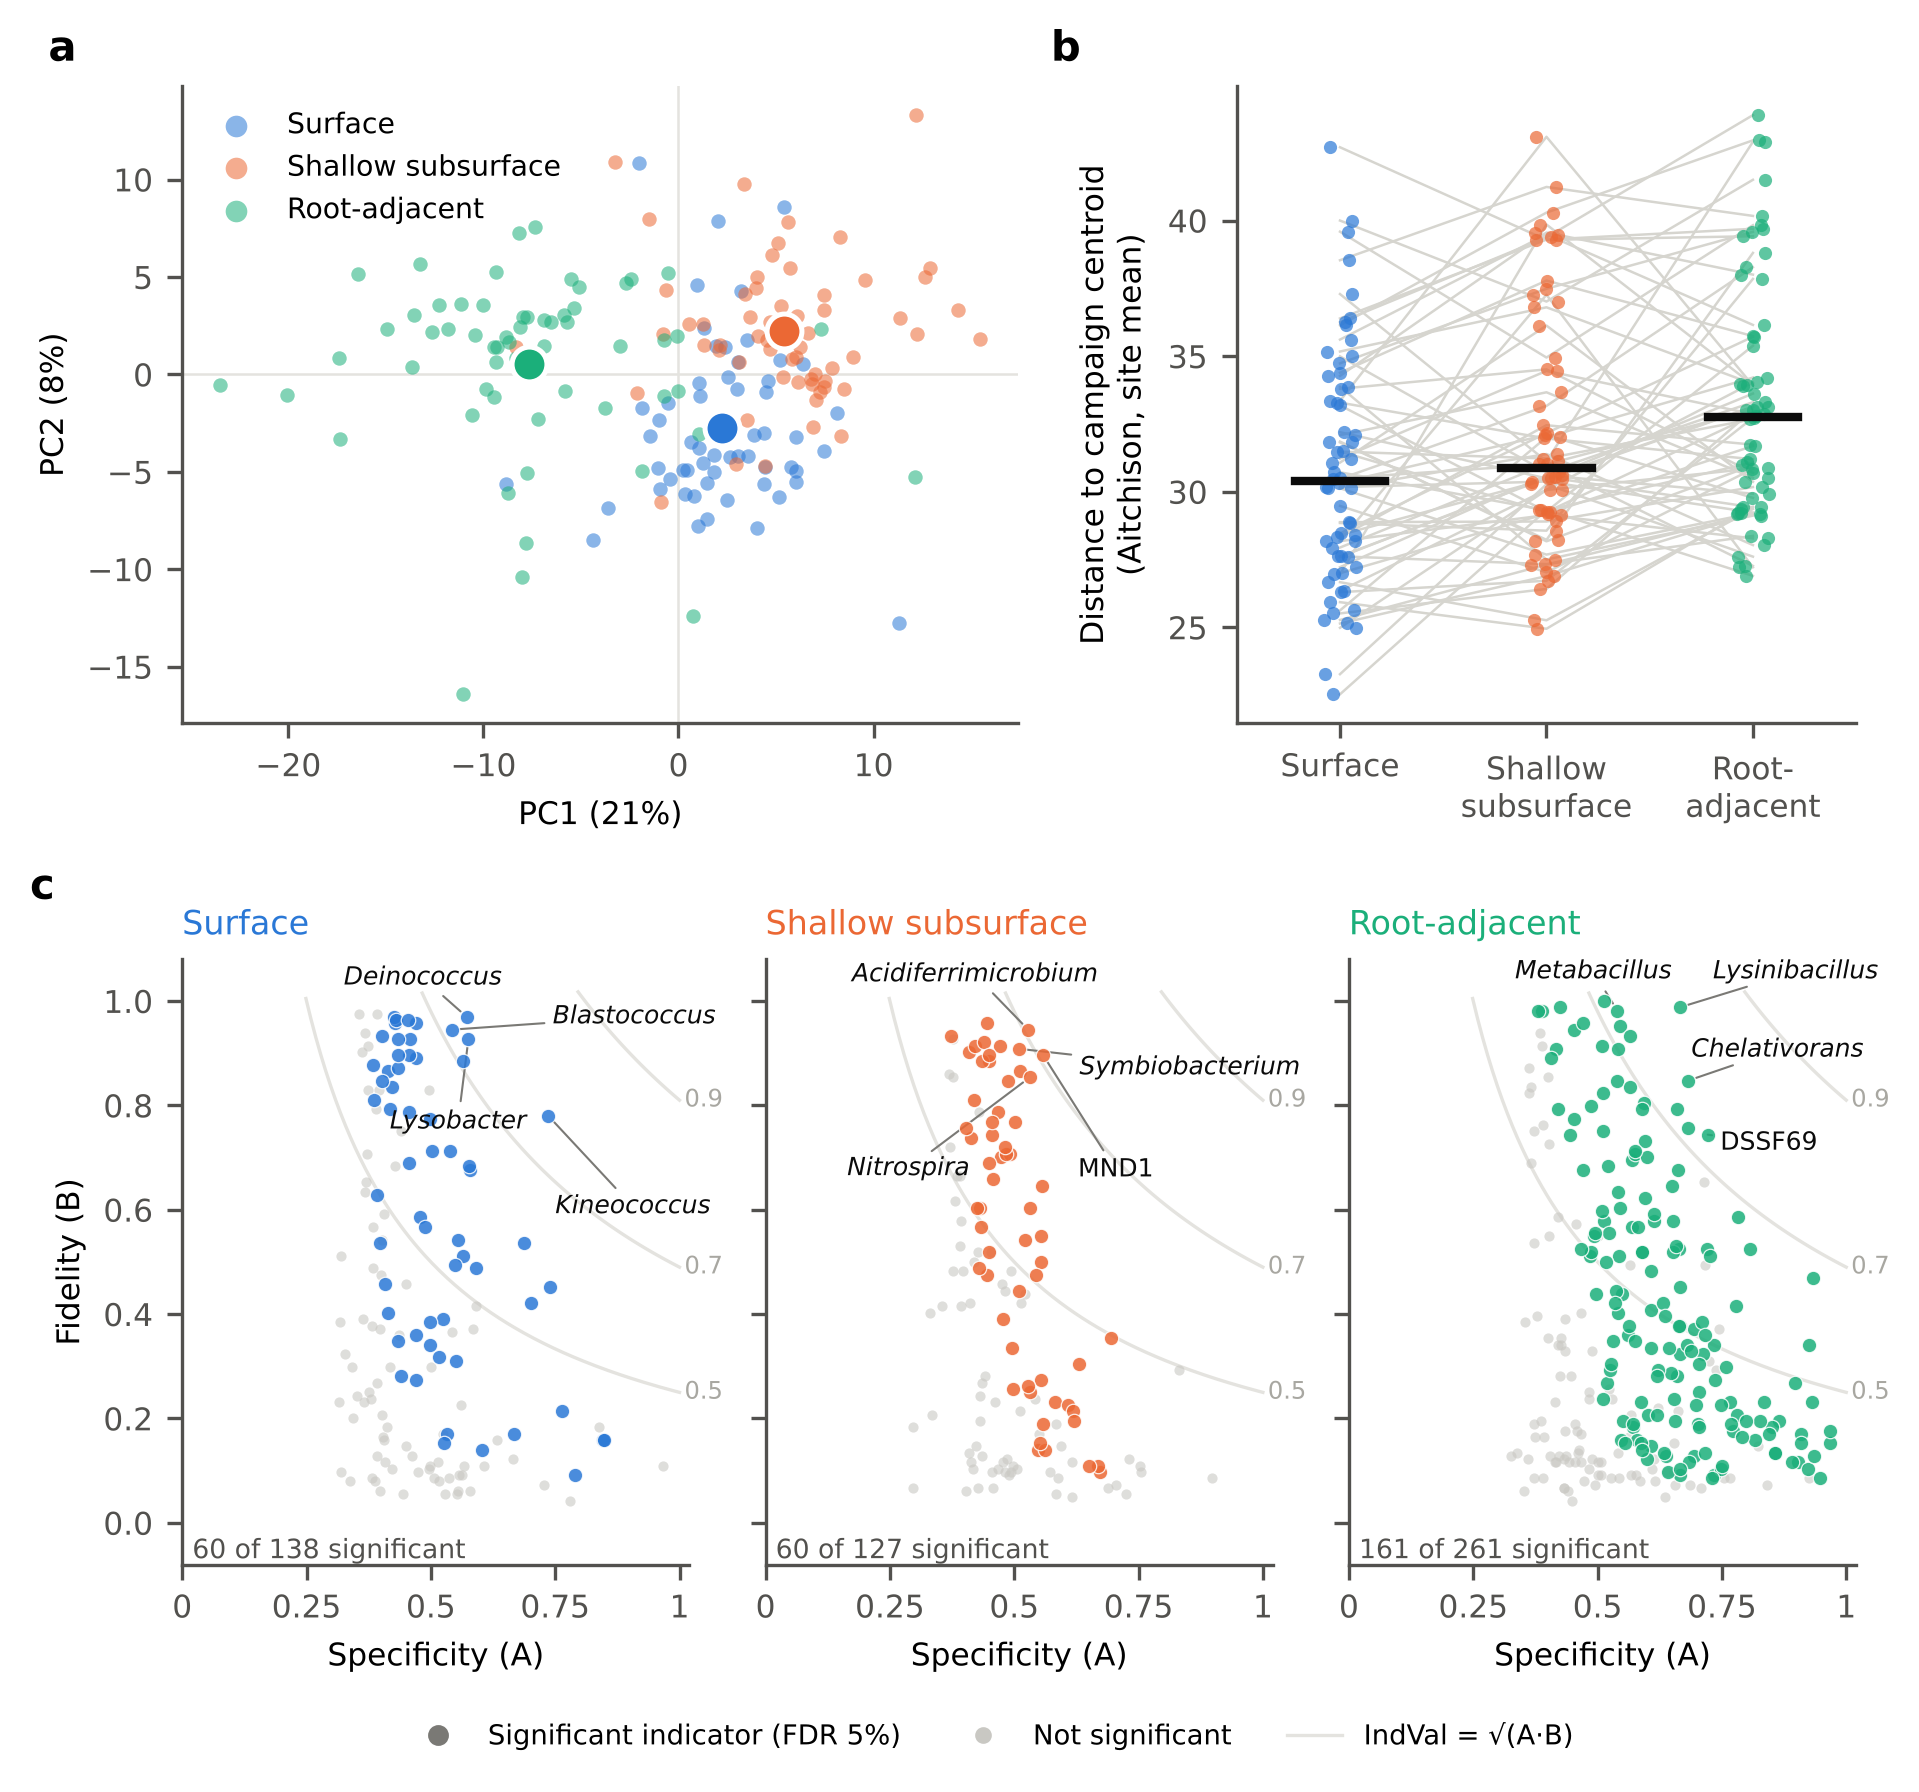
\includegraphics[width=\linewidth]{updated_figures/fig6_compartments.png}
\caption{Compartment differences in community composition within sites. (a) PCA of within-site compartment shifts. Small points are sites, and large points are compartment means. (b) Dispersion based on Aitchison distance. Lines link the three compartments of a site, and black bars show medians. (c) Indicator genera of each compartment.}
\label{fig:compartments}
\end{figure}

\subsection*{Surface enrichment of betaine uptake and peroxide defence accompanies community turnover}

To test whether the compartment differences observed in the amplicon survey extend to encoded metabolic and stress-response capacities, we first compared ecological contrasts inferred from PICRUSt2 with those derived from the 5,438 species-representative genomes (\texttt{EQ-MAG-\allowbreak REFINED-\allowbreak v1.0.0}) in the 442 exact specimen-matched libraries (\texttt{EQ-COVERM-\allowbreak REL-\allowbreak ABUND-\allowbreak v1.0.0}). Across 8,860 shared KOs normalised to each platform's complete KO total, surface--subsurface and root-adjacent--subsurface effect sizes were moderately correlated between methods (Spearman $\rho=0.52$, 95\% spatial-block CI $0.31$--$0.54$, and $\rho=0.55$, 95\% CI $0.43$--$0.57$, respectively), and their directions agreed for $67.0\%$ and $67.8\%$ of KOs (Supplementary Section~\ref{si-sup:mag_integration}). Because marker-gene prediction captured only part of the genome-resolved functional variation between soil compartments, we evaluated selected functional groups and their carriers directly in the shotgun metagenomes and recovered genomes.

We evaluated 41 published microTrait rules \cite{karaoz2022microtrait} using protein-profile searches on the 20,451,986 representative-genome proteins called by Pyrodigal (\texttt{EQ-PROT-\allowbreak PYRODIGAL-\allowbreak REP-\allowbreak v1.0.0}) and separately projected the rules onto the frozen analytical representative-genome KO matrix (\texttt{rep\_ko\_v2.tsv}; Methods and Supplementary Section~\ref{si-sup:mag_integration}). The panel distinguished compatible-solute uptake from de novo synthesis and acute exposure protection from baseline DNA maintenance. In paired comparisons across 68 visits at 36 sites, the mapped community had greater representation of the BetL glycine-betaine transporter (K02168) and the AhpCF peroxide-reduction system (K03386/K03387) at the surface than in shallow subsurface soil (Figure~\ref{fig:mag_functions}a). The mean surface excess was $7.6$ and $6.9$ percentage points, respectively. Both contrasts retained positive spatial-block intervals under the KO projection, with the original-read denominator, in higher-quality genomes ($\ge 70\%$ completeness, $\le 5\%$ contamination) and in the 442-library matched amplicon cohort across 58 sites. Spatial models across the 545 read-depth-annotated metagenomes adjusting for campaign, read depth and dune field supported the same directions ($+6.70$ percentage points, 95\% CrI $5.24$--$8.16$ for BetL; $+5.53$ percentage points, 95\% CrI $3.84$--$7.22$ for AhpCF; Supplementary Table~\ref{si-tab:mag_spatial}).

The full microTrait workflow on all 5,438 genomes retained these surface associations under a separate gene-calling and rule-processing implementation (\texttt{EQ-MICROTRAIT-\allowbreak REP-\allowbreak v1.0.0}; \cite{rubalkhali_datapaper}). In the same 68 paired visits, the estimated surface excess was about 6.9 percentage points for each trait, with positive spatial-bootstrap intervals under both mapped-community and original-read denominators (Supplementary Table~\ref{si-tab:microtrait_sensitivity}). The BetL contrast was slightly smaller than in the initial profile screen, whereas the AhpCF contrast changed little.

The broader 41-rule trait panel distinguished these associations from a uniform increase in stress-response genes. Surface communities also had greater representation of photolyase and carotenoid markers, whereas superoxide dismutase and betaine-biosynthesis contrasts remained uncertain. DNA-repair markers differed in their responses: mismatch repair was enriched at the surface, while base-excision repair showed little difference. Trehalose results depended on the annotation rule. The complete panel, including uncertain and annotation-sensitive results, is reported in Supplementary Table~\ref{si-tab:stage4_selected_panel}.

Using GTDB release 232 assignments, changes in community membership accounted for most of these contrasts: between-genus replacement contributed $5.9$ percentage points to the BetL difference and $5.3$ points to the AhpCF difference, changes within shared genera contributed less than $0.3$ percentage points in either direction, and the remainder came from groups detected in only one compartment (Supplementary Table~\ref{si-tab:canonical_turnover_3guilds}); the earlier taxonomy snapshot gave a similar decomposition (Figure~\ref{fig:mag_functions}b). Supplementary Section~\ref{si-sup:mag_integration} reports annotation-sensitive results, taxonomy-snapshot provenance and the treatment of genomes without genus assignments.

Genome-resolved profiles also identified archaeal populations beyond the bacterial focus of the amplicon survey, with Thermoplasmatota consistently more represented in shallow subsurface than in surface soil across paired sites (Supplementary Section~\ref{si-sup:mag_integration}). Detailed analyses of archaeal occurrence across the transect and the sequence-dark, export-enriched accessory proteome of these desert Thermoplasmatota are reported in the companion proteome study \cite{proteome_companion}.

\begin{figure}[!htbp]\centering
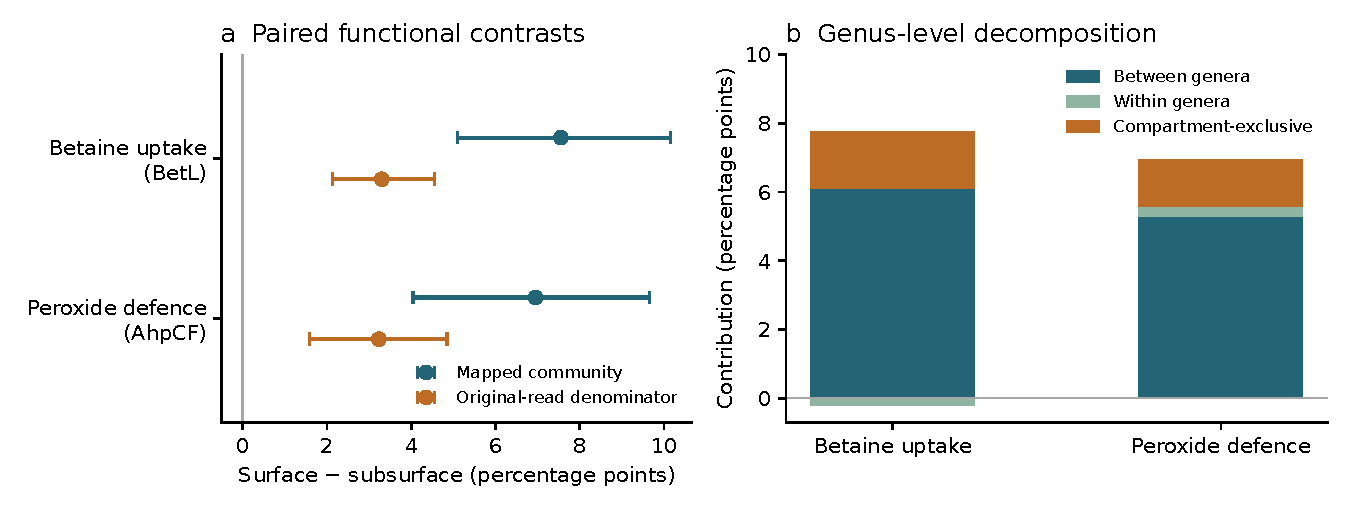
\includegraphics[width=\linewidth]{figures/functional_integration.pdf}
\caption{Surface-associated betaine uptake and peroxide defence accompany community turnover. (a) Mean surface-minus-subsurface differences across 36 sites contributing 68 paired visits. Intervals resample ten contiguous spatial blocks. Gene-content calls use the published BetL and AhpCF profile rules. (b) Exact decomposition into changes between shared genera, changes within those genera and compartment-exclusive contributions under the earlier taxonomy snapshot; the GTDB release 232 decomposition gives the same conclusion (Supplementary Table~\ref{si-tab:canonical_turnover_3guilds}). Replicates are averaged within visits and visit differences within sites. Unclassified genera enter as individual genomes.}
\label{fig:mag_functions}
\end{figure}

\subsection*{Root-adjacent communities have selectively reduced group 1l hydrogen-scavenging capacity}

Oxidation of atmospheric $\mathrm{H}_2$ and $\mathrm{CO}$ by high-affinity hydrogenases and carbon monoxide dehydrogenases is an established energy-conservation strategy supporting microbial persistence in desert soils \cite{ji2017atmospheric,cordero2019atmospheric,bay2021trace,bay2021aridity}. To test whether the distinct root-adjacent communities alter the representation of trace-gas-scavenging guilds across the Rub' al-Khali, we classified hydrogenase and carbon monoxide dehydrogenase large subunits by enzyme group, then quantified their representation directly in metagenomic reads relative to single-copy ribosomal genes. Across 106 depth-matched visits at 47 sites, group 1l $[\mathrm{NiFe}]$-hydrogenase (\texttt{HhyL}) representation was $4.8$-fold lower beside roots than in bulk subsurface soil (median $0.056$ versus $0.271$ genome equivalents; Figure~\ref{fig:loa_guilds}a). Its depletion exceeded the mean change in control hydrogenase and CoxL groups by $1.8$ log$_2$ units (95\% site-bootstrap interval, $1.0$--$2.6$ units of additional depletion; Figure~\ref{fig:loa_guilds}c). This excess persisted across campaigns, sequence-identity thresholds and contamination exclusions. Held-out sequence and simulated-community benchmarks supported recovery of the root-to-bulk contrast (Supplementary Section~\ref{si-sup:loa_methods}).

The spatial model across the 545 read-depth-annotated metagenomes retained the group 1l excess after accounting for campaign, read depth and dune field ($-1.733$ log$_2$ units, 95\% CrI $-2.038$ to $-1.424$; Supplementary Table~\ref{si-tab:mag_spatial}). Root-adjacent contrasts for groups 1h ($-0.083$ log$_2$ units, 95\% CrI $-0.213$ to $0.047$) and 2a ($0.052$ log$_2$ units, 95\% CrI $-0.083$ to $0.187$) were centred near zero. Form-I CoxL showed a small decrease in the spatial model ($-0.117$ log$_2$ units, 95\% CrI $-0.224$ to $-0.011$), whereas its paired contrast was uncertain (raw excess $+0.016$; Supplementary Section~\ref{si-sup:loa}). Group 1l therefore showed the strongest selective root-adjacent depletion. Surface soil had a broader reduction across all four high-affinity groups relative to the controls (Figure~\ref{fig:loa_guilds}b), distinguishing the surface and root-associated patterns.

This functional difference was primarily associated with lineage replacement. Across the 5,438-genome catalogue, the mean root-adjacent change in the mapped share of group 1l carriers was $-18.8$ percentage points: under GTDB release 232 assignments, changes between shared genera ($-11.6$ percentage points) and contributions from compartment-exclusive groups ($-6.8$ percentage points) accounted for almost all of this decrease, whereas the within-genus component was $-0.4$ percentage points, and the earlier taxonomy snapshot gave a similar decomposition (Supplementary Table~\ref{si-tab:canonical_turnover_3guilds}). In an exploratory analysis under the earlier taxonomy snapshot, genus carriage of group 1l remained associated with depletion beside roots after adjustment for predicted maximal growth potential (\texttt{gRodon2} \cite{weissman2021grodon}) and taxonomic order ($p \le 7.4\times 10^{-4}$; [PENDING: \texttt{TAXONOMY-\allowbreak SNAPSHOT-\allowbreak SENSITIVITY}; confirm order- and genus-adjusted \texttt{gRodon2} regression using canonical assignments]). Group 1l representation also declined as extract DNA concentration increased, including within visits and within bulk soil alone. Because extract DNA concentration combines microbial DNA, co-extracted plant DNA and extraction efficiency rather than measuring microbial biomass directly, and metagenomic marker representation measures encoded genetic capacity rather than in situ gas oxidation, this association describes relative guild representation along a DNA-yield gradient (Supplementary Figure~\ref{si-fig:loa_scaling}).

\begin{figure}[!htbp]\centering
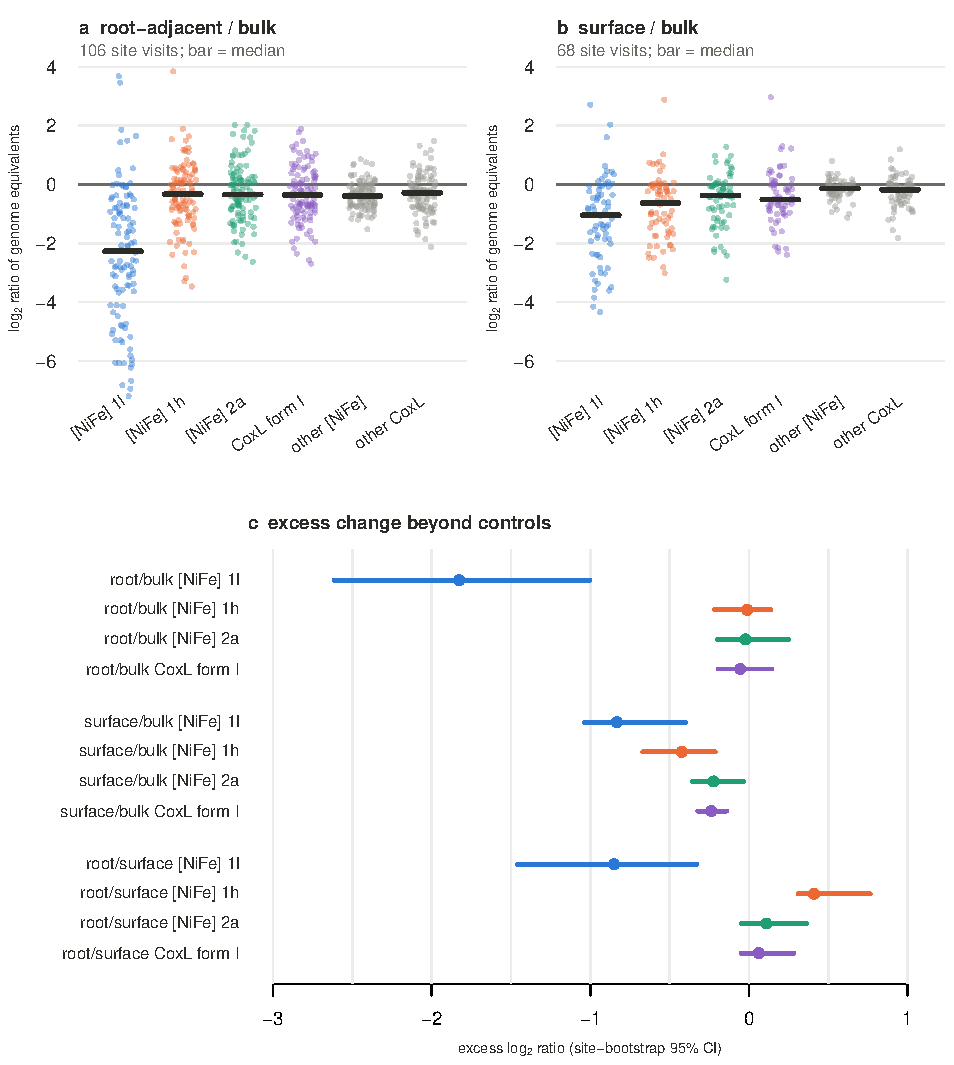
\includegraphics[width=\linewidth]{figures/loa_guilds.pdf}
\caption{Group 1l hydrogenase genes show strong selective depletion beside roots. (a) Log$_2$ ratios of estimated genome equivalents between root-adjacent and bulk subsurface soil at 5--10~cm, for 106 paired visits at 47 sites. (b) Surface versus subsurface soil, for 68 visits at 36 sites. Points are visits and bars are medians. (c) Excess log$_2$ ratios beyond the mean of the two control marker sets, with 95\% site-bootstrap intervals. These paired estimates are complemented by the spatial models in Supplementary Table~\ref{si-tab:mag_spatial}.}
\label{fig:loa_guilds}
\end{figure}


%%%%%%%%%%%%%%%

\subsection*{Bacterial diversity varies within sites across time and small spatial scales}
% \todo[inline]{Change header}
Bacterial diversity also varied within sites, both between campaigns and between soil compartments sampled during the same campaign. Variation between campaigns at the same site was about half that observed between sites along the transect (SDs of $\pm0.26$ and $\pm0.56$ in log richness, respectively). Variation between compartments within the same site and campaign (SD $\pm0.33$) was also high, indicating that the magnitude of diversity differences between compartments varied across sites and campaigns.

These within-site patterns were not explained by local variation in soil chemistry. Richness did not show a clear association with within-site variation in pH ($1.7\,\%$ per SD, $95\,\%$ CrI $-2.9$ to $6.6\,\%$) or elemental score ($-2.9\,\%$, $95\,\%$ CrI $-7.1$ to $1.5\,\%$), with both estimates excluding effects larger than approximately 7\% per standard deviation. Both Shannon diversity measures were also not associated with either soil property.

\subsection*{PMA-accessible DNA contributed to measured richness}

To assess the contribution of PMA-accessible DNA, we treated paired aliquots of three parent soil samples from two Trip~$5$ campsites with propidium monoazide (PMA), which suppresses amplification of extracellular DNA and DNA in membrane-compromised cells (Supplementary Section~\ref{si-sup:relic}). PMA-treated aliquots had lower rarefied richness than untreated aliquots in eight of the nine technical slurry pairs (18 libraries in total; Supplementary Figure~\ref{si-fig:relicRichness}). The mean reduction was $37$ ASVs in root-adjacent soil from the first campsite, $342$ in root-adjacent soil and $111$ in surface soil from the second campsite. Shannon diversity varied less consistently ($+0.73$, $-0.02$ and $-0.31$). Because each group comprised three technical slurries prepared from one biological parent soil tube, these comparisons describe the PMA response of those three parent samples rather than landscape-wide relic-DNA proportions.


\section*{Discussion}

\subsection*{The Empty Quarter microbial ecology}
Our survey shows that microbial communities across the Rub' al-Khali are structured at multiple spatial scales. Community composition changed gradually along the west-east transect, primarily through the replacement of genera between sites. The strongest differentiation occurred in the eastern megabarchan field, where bacterial richness was markedly lower and several genera associated with saline environments were relatively enriched. MAG profiles corroborated the eastern taxonomic decline, while annotated KO diversity showed a smaller contrast. Within sites, root-adjacent soil supported less diverse and compositionally distinct communities, while repeated sampling revealed substantial variation between visits. Together, these patterns show that the Rub' al-Khali soils support a mosaic of microbial habitats.

\subsection*{Landscape-scale turnover and the eastern megabarchan field}
Community dissimilarity increased with geographic distance in all three soil compartments, with genus replacement accounting for most of the differences between sites. This is consistent with biogeographic patterns reported in other deserts, including habitat-specific differences in the Namib \cite{ronca2015namib} and regional turnover along aridity gradients \cite{neilson2017significant}. Climate, pH, and elemental composition also varied along the transect, but these properties covaried with geographic position. We therefore interpret the distance decay pattern as evidence of landscape-scale structuring, rather than attributing it to any single environmental driver.

The eastern megabarchan field stood out from this broader pattern. Bacterial ASV richness was 79\% lower than in the western uruq field and genome-resolved bacterial MAG Hill diversity was 68\% lower, and several genera associated with saline environments, including \textit{Aquibacillus}, \textit{Sediminibacillus}, \textit{Halalkalibacter}, and \textit{Halomonas} were relatively enriched. These changes coincided with soil elemental scores of higher Ca, Mg, Na, S, and Cl relative to Si, consistent with higher evaporite influence. Although evaporite-rich soils were associated with lower diversity and greater compositional dissimilarity, these associations weakened after accounting for dune field. Annotated KO copy-number diversity showed a smaller east--west contrast than taxonomic diversity. The eastern decline therefore cannot be attributed to soil elemental composition alone. The megabarchan region also includes saline pans, oases and other surfaces, and our sampling cannot separate their contributions from those of the broader landscape transition.

% Although turnover was consistently positive, whether its rate differed between compartments remains unresolved. The apparent difference between shallow subsurface and root-adjacent soil was within the uncertainty of our estimates. Furthermore, the shape of the distance-decay relationship is less certain beyond approximately 500 km, where relatively few site pairs span the full transect. Nevertheless, the consistent increase in community dissimilarity with distance indicates that microbial communities are spatially structured across the Empty Quarter, despite the apparent continuity of its sandy landscape.

% \subsection*{Environmental filtering in the Eastern megabarchan field}

% The eastern megabarchan field exhibits differences from the broader landscape pattern . Richness was 79\% lower than in the uruq field, accompanied by substantial changes in the presence and abundance of individual genera. Several genera associated with saline environments, including Aquibacillus, Sediminibacillus, Halalkalibacter and Halomonas, were relatively enriched, whereas Aridibacter, Nocardioides and Rubrobacter were depleted. These compositional changes coincided with an elemental signature characterised by higher Ca, Mg, Na, S and Cl relative to Si, consistent with greater evaporite influence.

% The correspondence between soil elemental composition and the enrichment of salt-associated genera suggests that environmental filtering under increasingly saline conditions contributes to community differentiation in the eastern sand sea. This interpretation is consistent with the saline pans (\textit{sabkhas}) of the eastern Rub' al-Khali, which support microbial communities adapted to saline environments \cite{mckay2016sabkha}. However, the association between elemental composition and bacterial communities weakened after accounting for dune field. This indicates that the apparent chemical gradient is closely tied to broader landscape differences and that the contribution of individual soil elements cannot be isolated in our transect.

% Importantly, the eastern megabarchan field is not a uniform dune habitat. It encompasses saline pans, oases and other surfaces, each potentially providing different conditions for microbial colonisation and persistence. The particularly low diversity observed in this region may therefore reflect the combined effects of landscape position, evaporite-rich soils and habitat composition, rather than a response to megabarchan dunes alone. Our sampling also cannot establish whether the transition to lower diversity occurs abruptly at the boundary of the field or represents a steep but continuous decline towards the east.

% % Soil pH showed a weak negative association with richness, but the estimated effect was small relative to the uncertainty of the analysis. The absence of a clear association should not be taken as evidence that pH is ecologically unimportant. More broadly, the relationships between bacterial communities, salinity and mineral composition are consistent with observations from other desert soils \cite{horstmann2024,debbaghnour2025}. However, disentangling the effects of these soil properties from other environmental conditions will require sampling across independent gradients and a wider range of desert landscapes.

\subsection*{Soil compartments as distinct microbial habitats}
Differences between soil compartments show that microbial communities also vary over much shorter spatial distances than those separating sites across the transect. Root-adjacent soil had lower richness and Shannon diversity than bulk soil, a distinct community composition and greater compositional variation between sites. This contrasts with observations from the Namib, where rhizosheath soil supported greater diversity than surrounding soil \cite{marasco2022namib}. Plant-associated soil can provide locally favourable conditions through organic inputs and changes in moisture \cite{marasco2022namib}, but such effects may be limited under the extreme water scarcity of the Empty Quarter. Importantly, our root-adjacent samples were collected near roots rather than from a consistently defined rhizosphere, because soil attached to roots could rarely be recovered. The observed differences therefore identify a distinct root-associated microsite, but do not establish direct plant–microbe effects.

Diversity also varied between campaigns at the same site, with variation in log richness approximately half that observed between sites. This temporal variation, like the differences between compartments, was not explained by within-site variation in pH or elemental composition. The five campaigns provide repeated observations across 31 months, but not continuous seasonal coverage. Other local or time-varying conditions may therefore contribute to the observed variation.

The genome-resolved analysis connects these compartment differences to encoded capacities. Surface enrichment of betaine uptake and peroxide defence was supported by independent annotation approaches and accompanied in the broader panel by higher representation of photolyase, carotenoid and mismatch-repair markers rather than a uniform increase across all stress-response or housekeeping repair pathways; under the frozen analytical taxonomy, these shifts tracked genus replacement ([PENDING: \texttt{TAXONOMY-\allowbreak SNAPSHOT-\allowbreak SENSITIVITY}; confirm using canonical assignments]). This pattern is consistent with habitat sorting of organisms carrying surface-exposure protection and osmolyte-import capacities, although gene presence alone does not establish expression or stress tolerance. The recovery of Thermoplasmatota throughout the transect also extends the survey beyond bacterial communities; their greater representation in shallow subsurface soil places these archaea within the same habitat structure \cite{proteome_companion}.

The trace-gas analysis gives a more specific functional interpretation of the root-adjacent community. Group 1l hydrogenase genes were selectively depleted beside roots in both direct marker-read screening and total mapped carrier share; under the frozen analytical taxonomy, this depletion tracked genus turnover and persisted after accounting for predicted growth potential and taxonomic order ([PENDING: \texttt{TAXONOMY-\allowbreak SNAPSHOT-\allowbreak SENSITIVITY}; confirm using canonical assignments]). This pattern is consistent with a reduced relative contribution of this hydrogen-scavenging guild near roots, where organic substrates may be more available. We did not measure substrate supply or hydrogen consumption, however, and root proximity also changes moisture and other soil properties. Neither metagenomic representation nor extract DNA concentration establishes absolute population loss or a causal effect of plants. The smaller form-I CoxL decrease in the spatial model further suggests a graded response among trace-gas guilds rather than a response exclusive to group 1l.

\subsection*{Scope and implications}
Our findings should be interpreted in light of the study design. A single transect cannot fully separate geographic position from environmental properties and landscape type, even when spatial structure and sampling-design simulations are considered. XRF measurements describe total elemental composition rather than soluble salts or soil salinity directly. In addition, 16S profiles represent relative abundance, and genus-level analyses were restricted to the 200 most abundant genera. The small PMA experiment further suggests that accessible DNA can contribute to measured richness, but its limited number of parent soil samples does not allow this contribution to be quantified across the survey.

This study establishes a repeatedly sampled, landscape-scale baseline for bacterial communities across the Saudi Empty Quarter. The observed turnover, eastern differentiation and within-site variation provide a basis for future studies that pair microbial surveys with direct measurements of soil moisture, soluble salts, vegetation and microbial activity. Such measurements will help identify the environmental processes underlying the microbial patterns documented here.

The MAG analyses connect these community differences to encoded capacities: surface enrichment in betaine uptake and peroxide defence, and root-adjacent depletion of group 1l hydrogenase carriers, largely followed lineage replacement. Direct metagenomic marker profiling further identifies trace-gas scavenging as a functional component of the distinction between root-adjacent and bulk soil.

% \subsection*{A regional framework for the Arabian Peninsula}

% Earlier studies in the Arabian Peninsula established habitat-specific patterns at individual locations. An inland sabkha in the United Arab Emirates hosted a saline microbial mat \cite{mckay2016sabkha}, and studies in Saudi Arabia examined highland soils \cite{yasir2015elevation}, arid sites \cite{khan2020saudi}, soil crusts \cite{aslam2016rainfall}, and the root microbiomes of desert plants \cite{eida2018desertplants}. Our survey contributes an additional scale to this work; a landscape-scale transect with repeated sampling of three soil compartments over five campaigns.

% We found that soil in the open Empty Quarter is alkaline, which falls within the range reported for soils in Saudi Arabia \cite{khan2020saudi}. At AlUla, soil beneath fertility islands formed by desert plants hosted bacterial communities distinct from those in the surrounding bulk soil, which was also more alkaline \cite{maurice2023fertility}. In the Empty Quarter, pH increased from west to east, and its association with community composition was largely shared with geography. The small unique pH component and strong geographic covariance support a landscape-scale association with the sampled environmental gradient. Paired sampling of patches with vegetation and surrounding bulk soil would test whether local pH differences, such as those observed in AlUla, also shape composition at the scale of individual plants.

% Regional experiments also provide practical models for follow up studies. In soil crusts associated with \textit{Rhazya stricta}, biomass increased threefold within a week of watering \cite{aslam2016rainfall}, consistent with the early response window selected by our rainfall models. In Jizan and AlWahbah, host-resolved surveys found the strongest plant-associated differentiation in the root endosphere \cite{eida2018desertplants}. Our root-adjacent compartment, which differed from bulk soil and had the lowest alpha diversity, represents the soil end of this root--soil gradient. Post-rainfall sampling and comparisons among identified host plants would connect these regional observations.

% Our survey also provides a baseline for biodiversity monitoring in restoration in the region, and three of our results inform monitoring design. First, because turnover accounted for most of the dissimilarity between sites, no single site represents the regional community, and monitoring should retain broad geographic coverage. Second, because the three compartments differed in composition and alpha diversity, they should be sampled separately. Third, because root-adjacent communities had higher dispersion among sites than surface soil, they may require more replicates than bulk soil to detect change. Around rainfall events, the first days after rain offer a candidate window for additional sampling. The linked samples, environmental measurements, sequences, and analysis inputs make these comparisons reusable \cite{rubalkhali_datapaper}.


% \subsection*{Sampling constraints and tests of mechanism}

% All sites lie on a single west--east transect, along which climate, pH and soil chemical composition change together, and every campaign proceeded in the same direction. Geographic position is therefore confounded with collection order and time of day, and the environmental gradients cannot be separated from one another or from geographic distance. In addition, community composition remained spatially autocorrelated after accounting for the transect, and support for the transect trend depended on the assumed spatial covariance and independent-noise fraction. We therefore treat the transect model as a description of the sampled landscape. Future surveys could reverse the direction of travel between campaigns, add shorter transects crossing the main route where terrain allows, and install autonomous soil sensors at selected sites. These changes would help separate geographic, environmental, and collection time effects while retaining feasible routes through the dune interior \cite{edgell2006arabian}.

% The environmental measurements describe the soil samples indirectly. Climate summaries describe air, rather than soil, conditions, pH was measured on stored soil samples with uneven coverage of campaigns, and XRF measures total elemental composition rather than soluble ions or salinity \cite{elmoatassem2025pxrf}. Soil moisture, temperature, conductivity, and soluble-ion measurements would characterize water and salt exposure more directly. Similarly, the exact sampling depth and distance from root were not recorded, and host plants were not identified, so the compartments are defined by how samples were collected. Recording these fields would help separate plant-associated differences from shared habitat effects.

% We did not measure function. Pathway and gene abundances were predicted from $16$S profiles with PICRUSt2 or inferred from the gene content of MAGs, and describe metabolic potential rather than activity. PICRUSt2 predictions depend on how closely the sampled taxa resemble sequenced genomes, and the MAGs used to evaluate them mapped to a small fraction of whole-genome reads. Sequence-resolved validation of marker genes and functional profiles derived directly from metagenomic reads would extend this comparison to a larger fraction of each community. Measurements of proteins, metabolites, cell abundance, and process rates, such as trace-gas uptake, would connect the predicted mechanisms to microbial activity \cite{ray2023chemosynthesis,tribbia2026tracegas}.

% Control samples did not cover all campaigns and sample processing stages. Extraction blanks were only linked to specific batches, and the recovery of mock community controls was variable. Future surveys should sequence extraction and PCR blanks with every batch, include positive standards, and record DNA concentrations and pooling measurements alongside sequencing metadata \cite{fierer2025controls}.

% \subsection*{Conclusions}

% The Empty Quarter hosts a structured microbial landscape. Bacterial
% assemblages change across the west to east, mainly through turnover of genera, and compartments differ in composition and alpha diversity within sites. Climate, soil pH, and soil chemical composition covary with the geographic pattern, and predicted metabolic potential also follows the same geographic and compartment structure. Exploratory rainfall models identify the first days after rain as a window for event-based sampling. Together, the survey provides a regional baseline and specific hypotheses on geographic, plant-associated, and metabolic patterns for repeated surveys and experiments.

Our survey follows a single west--east transect, along which geographic position, climate, soil properties and landscape type covary. Although simulations based on the sampling design support the identification of associations with site-mean soil properties under random spatial variation, they cannot exclude all forms of spatial confounding. In addition, read counts represent relative rather than absolute abundance, extract DNA concentration reflects total recovered DNA rather than microbial biomass, and MAG gene content and metagenomic marker representation indicate encoded genetic capacity rather than measured metabolic activity. PICRUSt2 predictions agreed only moderately with MAG-based functional contrasts ($\rho=0.52$--$0.55$), reflecting reference-genome limits in hyperarid soils, while incomplete genomes and unmapped organisms constrain the genome-resolved analysis. Amplicon genus-level models were also restricted to the 200 most abundant genera. Together with the companion data resource \cite{rubalkhali_datapaper} and archaeal proteome study \cite{proteome_companion}, our findings show that microbial community assembly across the Rub' al-Khali operates primarily through lineage replacement across dune fields and soil compartments, reorganising encoded capacities for compatible-solute uptake, oxidative and photoprotective defence, and atmospheric trace-gas oxidation across the habitats of the sand sea.

%% ====================================================================
\section*{Methods}\label{sec11}

\subsection*{Study area}

We sampled 60 sites along a west to east transect covering over 1,000~km of the Empty Quarter of Saudi Arabia (Figure~\ref{fig:landscape}a). We repeated the sampling across five campaigns: 17-20 March 2023 (Trip 1), 14 July 2023 (Trip 2), 17–21 February 2024 (Trip 3), 29–31 August 2024 (Trip 4) and 12–15 October 2025 (Trip 5). All campaigns covered the 60 sites except Trip 2, which was restricted to eight sites due to extreme heat.

At each site, we sampled three soil compartments: bulk surface soil ($0\,\mathrm{cm}$), bulk subsurface soil, and subsurface soil we refer to as ``root-adjacent'' collected near plant roots ($5$--$10\,\mathrm{cm}$). Although we initially targeted the rhizosphere, most plants were so desiccated that the soil attached to the root could not be collected. We therefore collected soil as close to the root as possible, which in some cases included the rhizosphere. We collected three replicate samples per compartment by either scooping soil into sterile tubes directly or using a sterile plastic spoon. We kept samples at $-20\,^{\circ}\mathrm{C}$ in a portable freezer during each campaign and stored at $-80\,^{\circ}\mathrm{C}$ in the laboratory.

During each site visit we recorded air temperature, and where available, atmospheric pressure, and relative humidity. We also photographed each sampling site and classified it into one of seven landform categories based on field observations: sand dune, saline pan, oasis, gravel plain, dune slack, aeolian lake, or oil spill.

We assigned each site to one of four dune areas based on its geographic location in the dune classification and distribution map of Edgell \cite{edgell2006arabian}. The map distinguishes two major dune types along the transect. Linear dunes including uruq (singular \emph{irq}; Arabic for vein), seif, and sigmoidal and hooked dune subtypes. Crescentic dunes in our study area were of the megabarchan subtype. Each site was classified according to the dune type and subtype mapped at its location.

\subsection*{Soil properties and climate data}
\subsubsection*{Soil properties}
We measured pH from $767$ stored soil samples from all campaigns. Air dried soil was sieved to $\le 2$~mm and suspended in $0.01$~M CaCl$_2$ at a $1$:$2.5$ (w/v) ratio. The suspensions were mixed on a hula mixer for 30 min, and left to stand for an additional 30 min. We measured pH using an Accumet AB315 meter fitted with a Fisher Scientific Accumet electrode (cat. no.\ 13-620-112), which we calibrated at the start of each session and rinsed with Milli-Q water between measurements. We only retained measurements from sessions with a valid calibration defined as an electrode slope of $95$--$102\,\%$, and a pH $10$ buffer read-back of $9.9$--$10.1$ and a value within the physical range. This resulted in $712$ admitted measurements ([PENDING: \texttt{ECOL-PH-MODEL-\allowbreak INPUT-\allowbreak PROVENANCE}; reconcile the exact sample-level pH input subset passed to the 16S SPDE regressions against the 712 admitted measurement records in \texttt{EQ-PH-\allowbreak SHARED-\allowbreak v1.0.1} by measurement and sample key.]), and pH coverage was incomplete and non-random across campaigns.

We measured total elemental concentrations in 725 stored soil samples across all campaigns using a Vanta handheld X-ray fluorescence (XRF) analyzer in Fast Mode. we retained the 11 elements detected in at least 75\% of samples and applied a $\log(1+x)$ transformation. We then standardized element values within each campaign to reduce between-campaign differences. Finally, we performed principal component analysis (PCA) on the standardized values and used the first principal component as a composite elemental score for each sample.

\subsubsection*{Climate data from external sources}
Since the environmental measurements we obtained capture weather at a point in time, we supplemented them with climate data from external sources. For each site, we retrieved monthly air temperature, total rainfall, and relative humidity from the Open-Meteo historical API resource \cite{openmeteo}.
%We also obtained daily precipitation for each site from the NASA POWER \texttt{PRECTOTCORR} resource \cite{nasa_power_2024}, using complete calendar days preceding the sampling date.

\subsection{Sample processing}
\subsubsection*{DNA extraction and 16S rRNA gene sequencing and analysis}
\label{sec:methods_sampleprocessing}
We extracted $0.9$--$1.2\,\mathrm{g}$ of soil with QIAGEN PowerLyzer PowerSoil or DNeasy PowerSoil Pro kits. We amplified the V3--V4 region of the $16$S rRNA gene with the Bakt\_341F (\texttt{CCTACGGGNGGCWGCAG}) and Bakt\_785R (\texttt{GACTACHVGGGTATCTAATCC}) primers \cite{klindworth2013primers} following a two-step protocol \cite{illumina16S}. Samples without a visible product of the expected size were re-amplified with more template ($8\,\mu\mathrm{L}$, then $12\,\mu\mathrm{L}$), and samples without a product after three attempts were classified as failed. Indexed libraries were pooled by molarity and sequenced on an Illumina NovaSeq~6000 SP flow cell ($2\times250$-bp paired-end reads) at the Bioscience Core Lab in KAUST.

We processed reads with nf-core/Ampliseq v2.14.0 \cite{nfcore, ampliseq}, and used DADA2 to infer exact amplicon sequence variants (ASVs) and SILVA v138.2 \cite{silva} to assign taxonomy. This resulted in $351,472$ ASVs from $1,271$ samples including $24$ controls ($18$ extraction blanks and $6$ PCR no-template controls). We assessed contamination at different study stages following recommendations for low-biomass microbiome studies \cite{fierer2025controls} (Supplementary Section~\ref{si-sup:controls}, Table~\ref{si-tab:controls}). We excluded control samples, 10 samples that had $< 10,000$ reads ([PENDING: \texttt{ECOL-READ-CUTOFF-RECONCILIATION}; current manuscript text cites a $<10{,}000$ read cutoff whereas canonical data descriptors record ten profiles with $<1{,}000$ reads, including \texttt{T1Dr1} with 934 reads; source threshold under verification]), and only kept the deeper library for samples that were sequenced more than once, resulting in $1,186$ samples.


\subsubsection{Metagenome sequencing and analysis}
We sequenced 554 paired-end shotgun runs from 551 soil samples on Illumina NovaSeq~6000 and NovaSeq~X platforms, including duplicate runs for three samples. We removed low-quality reads using fastp v1.0.1 \citep{chen2018fastp} and assembled metagenomes with MEGAHIT v1.2.9 \citep{li2015megahit}; 549 samples yielded assemblies. We binned contigs using SemiBin2 v2.2.1 \citep{pan2023semibin2} with both pretrained and self-supervised models, and used DAS\_Tool v1.1.7 \cite{sieber2018dastool} to reconcile their outputs into 14,426 bins. CheckM2 v1.1.0 \citep{chklovski2023checkm2} identified 12,434 bins with at least 50\% completeness and at most 10\% contamination. We used dRep v3.6.2 \citep{olm2017drep} to dereplicate the resulting bins at primary and secondary ANI thresholds of 90\% and 95\%, resulting in 5,438 species representatives (4,847 bacterial and 591 archaeal).

We used GTDB-Tk v2.7.2 \cite{chaumeil2022gtdbtk} to taxonomically classify the genomes against GTDB release 232 \cite{parks2022gtdb}. Gene calling used Pyrodigal v3.7.1 in metagenomic mode (\texttt{EQ-PROT-PYRODIGAL-REP-v1.0.0}), distinct from the companion Bakta release annotation product (\texttt{EQ-PROT-BAKTA-v1.0.0}; see companion methods \cite{rubalkhali_datapaper} and Section~\ref{methods:mag_lifeonair}). We estimated genome abundances using CoverM v0.7.0 \cite{aroney2025coverm}. Functional analyses use 442 sample profiles across 58 sites that match the 1,186 samples from the 16S rRNA gene cohort.



\subsection*{Statistical analysis}
\subsubsection*{Hierarchical model}
Replicates from the same site, campaign and compartment are not independent. We therefore analyzed sample-level responses using Bayesian hierarchical models fitted with integrated nested Laplace approximation (INLA) \cite{rue2009}. Fixed effects were compartment, campaign, and sequencing run. Random effects were site $\times$ campaign $\times$ compartment groups, nested within site visits (sites $\times$ campaigns) and sites, so that replicates entered as repeated measurements of their group.

Spatial dependence between sites was modeled with a Matérn field ($\nu = 1$) over site coordinates using the stochastic partial differential equation (SPDE) approach \cite{lindgren2011}. The standard deviations (SDs) of the random effects had penalized complexity (PC) priors with $P(\mathrm{SD} > 1) = 0.01$ \cite{simpson2017penalising}. The spatial field had PC priors with a prior median range of 200~km and $P(\sigma > 1) = 0.01$ \cite{fuglstad2019constructing}. Covariates were standardized. All fixed effects except the intercept had normal priors with mean 0 and SD 1 in the diversity models, and SD 10 in the genus models. The intercept had a flat prior. Posterior distributions were computed with INLA's default integration over the hyperparameters. Sensitivity to the priors was assessed with prior median ranges of 50 and 500~km, and with the SD prior scales halved and doubled (Supplementary Section~\ref{si-priors}; Supplementary Table~\ref{si-tab:prior_sensitivity}).



\subsubsection*{Alpha diversity}
We used three measures of within-sample diversity. Shannon diversity ($H$, natural logarithm) was calculated at full read depth as it is less sensitive to variation \cite{shirazi2021revisiting}. Rarefied richness was estimated as Hurlbert's expected number of ASVs at $25{,}000$ reads ($E[S_{25k}]$), which controls for sequencing depth \cite{hurlbert1971nonconcept}. This threshold is near the $5$th percentile of sample library size (median $382{,}432$ reads per sample), and approximately 5\% of libraries were excluded from richness analyses. To measure abundance relative to rarefied richness, we used a normalized Shannon index $H/\log(E[S_{25k}])$.



We modeled log rarefied richness, Shannon diversity and normalized Shannon diversity with a Student-$t$ likelihood (10 degrees of freedom) which accommodates the heavy lower tail of residuals from a subset of samples with very low diversity.
%Estimating the degrees of freedom, or fixing them at 3, gave unstable fits; models with Gaussian and Student-$t$ (5 degrees of freedom) likelihoods were fitted as sensitivity analyses (Supplementary Section~\ref{X}).
Models for Shannon and normalized Shannon diversity included standardized log read depth as a fixed effect. Rarefied richness effects are reported as percentage changes per SD of the predictor, and Shannon and normalized Shannon effects as differences in index units.


\subsubsection*{Community composition}
We summarized taxonomic composition as the mean relative abundance of phyla, classes and genera (unclassified reads retained) across all samples, by compartment and by dune zone \cite{edgell2006arabian}.

% \paragraph{Indicator genera}
% We identified genera associated with soil compartments and dune fields using the group equalized indicator value (IndVal.g; \cite{dufrene1997species}). Each genus was assigned to the group with the highest indicator value. For compartments, we summed reads within each site, campaign and compartment, rarefied to $20{,}000$ reads, and retained the $164$ visits sampled in all three compartments ($492$ samples). We analysed $526$ genera present in at least $5\,\%$ of samples, permuting compartment labels within visits. For dune fields, we pooled libraries within sites, rarefied to the smallest site total, and analysed $1{,}149$ genera present at three or more sites. We permuted contiguous blocks of five sites along the transect to account for spatial dependence. Significance was assessed using $9{,}999$ permutations and false discovery rates controlled at $5\,\%$.

\paragraph{Dissimilarity}
For abundance-based dissimilarity, we summed replicates for each site $\times$ campaign $\times$ compartment group, and discarded profiles with fewer than 2,000 reads (630 groups across 60 sites). We applied a centered log-ratio (CLR) transformation of the 200 genera after adding a $0.5$ pseudocount. Aitchison distance, the Euclidean distance between CLR profiles, was used to compare genera through their abundance ratios \cite{tellmewhy}. For presence--absence dissimilarity, we pooled counts within site $\times$ compartment groups across campaigns, and rarefied each pooled profile to 12,863 reads (smallest pooled library). Sørensen dissimilarity was calculated as the mean over 20 rarefactions. We calculated Sørensen dissimilarity as the mean over 20 rarefactions, and partitioned it into turnover (Simpson dissimilarity, the replacement of genera) and nestedness (the loss of genera) components \cite{baselga2010partition}, using the R package \textit{betapart}.

\paragraph{Distance decay}
Pairwise dissimilarities are not independent observations, so we analyzed distance decay separately from the hierarchical models. For Aitchison distance, we centered each CLR profile by subtracting the mean profile for its campaign $\times$ compartment group, then averaged the centered profiles within each site and compartment. Within each compartment, we regressed pairwise Aitchison distance on geographic distance using multiple regression on distance matrices and report slopes per 100~km. We applied the same approach to Sørensen dissimilarity and its turnover and nestedness components.

To select interval methods, we simulated communities on our site layout from Gaussian processes with ranges of 300 and 1,000~km (Supplementary Section~\ref{si-decay_calibration}). Delete-one-site jackknife intervals recovered the true slope in only 82\% and 67\% of 500 simulated datasets, and intervals from a model with random effects for both sites in each pair in only 11–12\% of 100 (Supplementary Section~\ref{si-decay_calibration}). We therefore calculated 95\% intervals with a block jackknife, sequentially deleting each of 12 contiguous blocks of five sites along the transect. These intervals covered the true slope in 94--100\% of simulations, but the true difference between two compartments' slopes in only 77--81\%, so differences between compartments should be interpreted with caution. Interval calibration was assessed for Aitchison distance only. To describe the shape of the decay beyond a linear trend, we fitted a smooth distance--response function with INLA, including random effects for both sites in each pair, and compared it with generalized dissimilarity modeling \cite{ferrier2007}. Because its intervals were poorly calibrated, and few site pairs span more than about 500~km, we use these curves descriptively.


\subsubsection*{Compartment differences}
Differences in diversity between compartments were estimated as contrasts between compartments in the models without environmental variables (Supplementary Section~\ref{si-models}). Differences in genus presence and abundance were estimated in the same way as the genus hurdle models, on both the raw and the relative scale, with the false discovery rate controlled separately for each model part, contrast, and scale. We used each compartment's CLR profile , and tested overall differences between compartments with PERMANOVA (999 permutations restricted within sites), pairwise differences with paired sign-flip tests, and differences in multivariate dispersion with sign-flip tests on each sample's distance to its campaign $\times$ compartment centroid, averaged within each site. P-values for the pairwise tests were adjusted for multiple testing using Benjamini--Hochberg. Restricting permutations and sign flips to within sites preserved the site-level structure and avoided exchanges between spatially separated sites.

\subsubsection*{Genus models}
We summed ASV counts by genus and analyzed genera with two complementary approaches. Hurdle models estimated the response of each genus separately to compartment and to site-level and within-site soil properties (Supplementary Section~\ref{si-hurdle}). A joint model of the most abundant genera estimated which genera varied together after accounting for the design and the environmental gradient (Supplementary Section~\ref{si-joint}).


\subsection*{Relic-DNA removal experiment}
PMA treatment suppresses amplification of accessible DNA, including extracellular DNA and DNA in membrane-compromised cells \cite{wang2021pma,sun2023,carini2017relic}. We prepared three separate technical soil slurries from each of three biological parent soil tubes collected at two T5 campsites (nine paired slurries, 18 libraries in total): root-adjacent soil at C1 and C2, and surface soil at C2. Each slurry was homogenized in sterile phosphate-buffered saline (PBS, pH $7.4$) at a $1:10$ (w/v) ratio and split into treated and untreated aliquots. We added PMAxx (Biotium, Hayward, USA) to treated aliquots at a final concentration of $50\,\mu\mathrm{M}$. Both aliquots underwent a 10 min dark incubation, photoactivation with a $450\,\mathrm{nm}$ LED lamp for 35 min on a white reflective surface ($15$--$20\,\mathrm{cm}$ from the lamp), and rotation at 15 min intervals. We stored samples at $-20\,^{\circ}\mathrm{C}$ until DNA extraction, which was performed using $860\,\mu\mathrm{L}$ from each aliquot with the DNeasy PowerSoil Pro kit (QIAGEN). We amplified the DNA and sequenced the samples with the protocols described in Section~\ref{sec:methods_sampleprocessing}.




\subsection*{Genome-resolved functional analysis}
\label{methods:mag_lifeonair}
{\emergencystretch=3em
Shotgun metagenomes from the same collection (551 read-bearing libraries, \texttt{EQ-\allowbreak SHOTGUN-\allowbreak READ-\allowbreak LIBS-\allowbreak v1.0.0}, sequenced across 554 paired-end runs on Illumina NovaSeq~6000 [221 runs] and Illumina NovaSeq~X [333 runs] instruments) were assembled with MEGAHIT and binned with SemiBin2; DAS\_Tool reconciled bins, CheckM2 assessed quality, and dRep grouped 12,434 retained bins at 95\% average nucleotide identity \cite{li2015megahit,pan2023semibin2,sieber2018dastool,chklovski2023checkm2,olm2017drep}. The resulting catalogue of 5,438 species-representative genomes (\texttt{EQ-\allowbreak MAG-\allowbreak REFINED-\allowbreak v1.0.0}) met completeness $\ge 50\%$ and contamination $\le 10\%$, comprising 126 high-quality and 5,311 strict medium-quality genomes ($<10\%$ contamination) under MIMAG standards plus one boundary representative (\texttt{48Dr2\_\_\allowbreak self\_\allowbreak SemiBin\_25}, $64.61\%$ completeness and $10.0\%$ contamination). In the foundational data release, GTDB-Tk classified the genomes against GTDB r232 (\texttt{gtdb\_\allowbreak r232\_\allowbreak classification}), and Bakta v1.12.0 and eggNOG-mapper v2.1.13 supplied the release gene annotations (\texttt{EQ-\allowbreak PROT-\allowbreak BAKTA-\allowbreak v1.0.0}, 19,186,792 proteins). CoverM v0.7.0 estimated genome abundances by competitive read mapping (\texttt{EQ-\allowbreak COVERM-\allowbreak REL-\allowbreak ABUND-\allowbreak v1.0.0}). After excluding one library with zero mapped reads (\texttt{F5Dr1}, $100\%$ unmapped; leaving 550 mapped libraries) and four out-of-core libraries from Sites~62 and 64 (\texttt{62PRr2}, \texttt{64Dr3}, \texttt{64PRr2} and \texttt{64Sr2}), the functional analysis retained 546 core-transect profiles across 59 sites (489 unique specimen keys; \texttt{EQ-\allowbreak ECOL-\allowbreak SHOTGUN-\allowbreak CORE-\allowbreak 546-\allowbreak v1.0.0}); exact specimen matching to the 1,186-sample amplicon cohort identified 442 retained libraries across 58 sites (\texttt{EQ-\allowbreak ECOL-\allowbreak MATCHED-\allowbreak 442-\allowbreak v1.0.0}). Supplementary Section~\ref{si-sup:mag_integration} defines cohort exclusions, genome-quality sensitivity and the competitive archaeal mapping checks (\texttt{EQ-\allowbreak COVERM-\allowbreak ARCHAEA-\allowbreak COMP-\allowbreak v1.0.0}).

We searched 20,451,986 representative-genome proteins called by Pyrodigal (\texttt{EQ-\allowbreak PROT-\allowbreak PYRODIGAL-\allowbreak REP-\allowbreak v1.0.0}) against 106 microTrait profiles at their published trusted cutoffs and evaluated 41 published rules \cite{karaoz2022microtrait}. A separate KO projection used the frozen analytical representative-genome KO matrix (\texttt{rep\_\allowbreak ko\_\allowbreak v2.tsv}, \texttt{EQ-\allowbreak KO-\allowbreak LEGACY-\allowbreak ANALYTICAL-\allowbreak v0}; IBEX \texttt{04\_\allowbreak functional/\allowbreak repko\_\allowbreak clean/\allowbreak results}) to assess dependence on annotation method; neither \texttt{EQ-\allowbreak PROT-\allowbreak PYRODIGAL-\allowbreak REP-\allowbreak v1.0.0} nor \texttt{rep\_\allowbreak ko\_\allowbreak v2.tsv} is asserted to derive from the 19,186,792-protein foundational Bakta release product (\texttt{EQ-\allowbreak PROT-\allowbreak BAKTA-\allowbreak v1.0.0}; [PENDING: \texttt{DATA-\allowbreak PROVENANCE-\allowbreak UNVERIFIED-\allowbreak PROTEIN-\allowbreak EQUIVALENCE}; verify upstream gene-caller and mapper provenance of the 20,451,986 Pyrodigal protein set and frozen \texttt{rep\_\allowbreak ko\_\allowbreak v2.tsv} matrix relative to the 19,186,792-protein Bakta release product]). Genome trait calls were weighted by abundance, with both the mapped-community and original-read denominators retained. For paired compartment contrasts, we averaged replicates within each site, visit and compartment and then averaged paired visit differences within sites. Confidence intervals resampled ten contiguous geographic blocks. An exact genus-level decomposition separated changes between shared genera, changes within shared genera and compartment-exclusive contributions. Whereas total trait contrasts and bacterial MAG Hill diversity are unaffected by sub-domain taxonomy labels, 1,898 full taxonomy strings (including 1,124 genus and 220 order labels) differ between the frozen analytical taxonomy snapshot (\texttt{EQ-\allowbreak TAX-\allowbreak LEGACY-\allowbreak ANALYTICAL-\allowbreak v0}, \texttt{genome\_\allowbreak quality.tsv}) used in the broad 41-trait matrix and canonical \texttt{gtdb\_\allowbreak r232\_\allowbreak classification} in \texttt{EQ-\allowbreak MAG-\allowbreak REFINED-\allowbreak v1.0.0}. For the three focal guilds (BetL, AhpCF and group 1l $[\mathrm{NiFe}]$-hydrogenase), the complete genus-turnover decomposition was rerun under canonical \texttt{gtdb\_\allowbreak r232\_\allowbreak classification} against the immutable legacy baseline using the identical abundance matrices, trait calls and paired visit sets, with 1,000 resamples across the ten contiguous spatial blocks (seed \texttt{20261108}) and individual-site resampling as a secondary sensitivity check, while retaining the frozen paired trait intervals from the original 1,000- and 2,000-draw analyses (Supplementary Table~\ref{si-tab:canonical_turnover_3guilds}). PICRUSt2 and MAG-derived KO profiles (\texttt{rep\_\allowbreak ko\_\allowbreak v2.tsv}) were normalised separately to their full KO totals and compared on the 442 exact specimen-matched libraries across 8,860 shared KOs, using the same paired design.
\par}

Functional responses and genome-community summaries were analysed with an adaptation of the spatial hierarchy above, using campaign, compartment and standardised log read depth as fixed effects, with and without dune field. The model retained site, site--visit and site--visit--compartment random intercepts and the two-dimensional Mat\'ern field. Responses were standardised before fitting a Student-$t$ likelihood with ten degrees of freedom; coefficients were transformed back to their analysis scale. One metagenome (\texttt{F45PRr3}) lacked read-depth metadata in the covariate table, leaving 545 profiles for these models (\texttt{EQ-ECOL-\allowbreak SHOTGUN-\allowbreak MODEL-\allowbreak 545-\allowbreak v1.0.0}) and 441 in the matched-cohort sensitivity (\texttt{EQ-ECOL-\allowbreak MATCHED-\allowbreak MODEL-\allowbreak 441-\allowbreak v1.0.0}). Sensitivities varied the spatial-range prior, likelihood and genome-quality restriction. These functional fits used the available spatial and sampling metadata; chemistry covariates were confined to the amplicon models. Numerical diagnostics and exclusions are reported in Supplementary Section~\ref{si-sup:mag_integration}.

\subsection*{Trace-gas oxidation genes and their carriers}

Hydrogenase large subunits were typed against HydDB, and CoxL proteins were classified using form-specific motifs and reference alignments \cite{sondergaard2016hyddb,cordero2019atmospheric}. We quantified groups 1l, 1h and 2a and form-I CoxL separately. Other [NiFe]-hydrogenases and other CoxL sequences supplied control groups. Ten million forward reads per library were sampled and truncated to 100 nt before competitive translated searches against the marker references and 14 universal single-copy ribosomal proteins. Length-normalised marker counts divided by median ribosomal-protein coverage defined genome equivalents. The primary analysis required 60\% amino-acid identity and detection of at least ten ribosomal markers. Excess compartment effects were the marker log$_2$ ratio minus the mean log$_2$ ratio of the two control sets.

Paired trace-gas contrasts used replicate medians within visits, site-level resampling and multiplicity adjustment within declared test families. Hierarchical spatial fits also analysed sample-level log$_2$(genome equivalents + 0.01) and excess-marker responses. Genus-level and order-adjusted analyses related carrier depletion to predicted maximal growth potential from gRodon2 and taxonomic order \cite{weissman2021grodon} under the frozen analytical taxonomy snapshot (\texttt{EQ-TAX-\allowbreak LEGACY-\allowbreak ANALYTICAL-\allowbreak v0}; [PENDING: \texttt{TAXONOMY-\allowbreak SNAPSHOT-\allowbreak SENSITIVITY}; confirm order- and genus-adjusted \texttt{gRodon2} regression using canonical assignments]). Supplementary Section~\ref{si-sup:loa_methods} gives the complete classification, read-assignment benchmarks, contamination controls, growth models and sensitivity analyses. These functional hypotheses were developed after inspecting the observational data.

\subsection*{Full microTrait annotation sensitivity}

We used the complete microTrait profiles of the shared 5,438-genome resource \cite{rubalkhali_datapaper,karaoz2022microtrait} to assess dependence of the two focal surface associations on annotation implementation. This workflow called genes with Prodigal v2.6.3 in metagenomic mode and applied the pinned microTrait profiles, coverage filters and logical rules. BetL required its transporter profile; AhpCF required an AhpC profile together with AhpF. We joined the resulting calls by exact canonical genome identifier to the same CoverM matrix and compared them with the earlier profile-based calls. For each annotation, we averaged replicate profiles within site, visit and compartment, calculated surface-minus-subsurface differences within visits, and averaged these differences within sites. We retained the same 68 visits at 36 sites, used 1,000 bootstrap resamples of ten contiguous transect blocks (seed 20261108), and reproduced the earlier estimates and intervals before evaluating the new calls. Mapped-community and original-read denominators were kept separate. This analysis is an annotation sensitivity check; the earlier INLA spatial-model estimates retain their original trait inputs. The complete rule matrices, gene-call provenance, missing-model flags and continuous predictions are documented in the data descriptor. The specialised group 1l hydrogenase classification and separate gRodon2 analyses retain their own inputs and methods.


\section*{Data availability}
Raw $16$S rRNA gene amplicon reads are deposited in the European Nucleotide Archive (ENA) under study accession \texttt{PRJEB106069}, part of the umbrella project \texttt{PRJEB104209} (public release scheduled for 25 November 2026). Sample, field, climate, soil pH and XRF metadata, the processed ASV tables and their provenance are available in the data repository of the companion data descriptor \cite{rubalkhali_datapaper} at \href{https://github.com/bio-ontology-research-group/empty-quarter-ecology-data}{the shared data repository}. The Empty Quarter knowledge graph (KG v3.0.1) is archived at Zenodo (\href{https://doi.org/10.5281/zenodo.23134168}{doi:10.5281/zenodo.23134168}); the bulk sequence and annotation archive for the 5,438 representative genomes (\texttt{EQ-MAG-\allowbreak REFINED-\allowbreak v1.0.0} and \texttt{EQ-PROT-\allowbreak BAKTA-\allowbreak v1.0.0}) is staged for Zenodo deposition ([PENDING: \texttt{DATA-\allowbreak BULK-\allowbreak ARCHIVE-\allowbreak DOI}; add the Zenodo DOI for the 5,438-MAG bulk sequence and Bakta annotation archive upon deposit]) \cite{rubalkhali_datapaper}. Analysis inputs, code, result tables and figure-generation scripts for this paper are available at \href{https://github.com/bio-ontology-research-group/empty-quarter-ecology}{the ecology reproducibility repository}.

Shotgun metagenomes have ENA study accession \texttt{PRJEB125153}; the companion resource records schedule public release for 25 November 2026. Genome-resolved integration coefficients, fit diagnostics, paired functional contrasts and their analysis scripts are provided in Supplementary Data~1 and the reproducibility repository. The trace-gas analysis code and benchmark inputs are maintained in \href{https://github.com/bio-ontology-research-group/empty-quarter-lifeonair}{the Life-on-air analysis repository}.

\subsection*{Reproducibility}
The companion data descriptor covers the field, specimen, amplicon,
environmental, XRF and knowledge-graph resources \cite{rubalkhali_datapaper}.
Inputs, scripts, machine-readable results, random seeds and checksums are
maintained in the dedicated reproducibility repository at
\href{https://github.com/bio-ontology-research-group/empty-quarter-ecology}{the ecology reproducibility repository}.
The repository links each analysis to its exact input, machine-readable result,
random seed and checksum, and links shared data products to the companion
resource. The shared knowledge graph, KG v3.0.1, is archived at
\href{https://doi.org/10.5281/zenodo.23134168}{Zenodo} with its original modules,
asserted export and rebuild kit. The public repository provides the staged
inputs and downstream analyses, including the corrected Site~52 rainfall
packages shared with the data descriptor. Its release checklist identifies
the upstream amplicon, PMA, shotgun-read and genome resources and execution
records required for a complete raw-read replay.

\subsection*{Software}
{\emergencystretch=3em
Amplicon reads were processed with nf-core/Ampliseq v2.14.0 (Nextflow; DADA2
and SILVA v138.2) on the KAUST Ibex cluster. In the companion data release, the 5,438 refined representative
genomes (\texttt{EQ-\allowbreak MAG-\allowbreak REFINED-\allowbreak v1.0.0}) are annotated with Bakta v1.12.0 and
eggNOG-mapper v2.1.13 (\texttt{EQ-\allowbreak PROT-\allowbreak BAKTA-\allowbreak v1.0.0}, 19,186,792 proteins),
whereas the functional integration in this paper searched the 20,451,986 Pyrodigal
representative-genome protein predictions (\texttt{EQ-\allowbreak PROT-\allowbreak PYRODIGAL-\allowbreak REP-\allowbreak v1.0.0}) and evaluated KO projections from the frozen analytical representative-genome KO matrix (\texttt{rep\_\allowbreak ko\_\allowbreak v2.tsv}, \texttt{EQ-\allowbreak KO-\allowbreak LEGACY-\allowbreak ANALYTICAL-\allowbreak v0}; [PENDING: \texttt{DATA-\allowbreak PROVENANCE-\allowbreak UNVERIFIED-\allowbreak PROTEIN-\allowbreak EQUIVALENCE}]);
an earlier 991-MAG, 150-library pilot annotated with eggNOG-mapper v2.1.12 is
retained only as a superseded historical archive (\texttt{EQ-\allowbreak COVERM-\allowbreak LEGACY-\allowbreak 991-\allowbreak v0}).
All statistical analyses
were run on a Linux workstation in Python v3.11.14 with pandas v2.2.3, NumPy
v2.1.3, SciPy v1.14.1, statsmodels v0.14.6, scikit-learn v1.5.2, scikit-bio
v0.7.3 and Biopython v1.84, together with R and R-INLA for spatial and
distance-decay models; PICRUSt2 v2.4.1 predicted functional potential.
Figures were drawn with Matplotlib v3.9.4 (FreeType v2.14.3). The complete
environment is pinned as a conda lock file with hashed pip requirements in the
reproducibility repository. Its tests check selected numerical calculations,
input/output consistency and manuscript values. A complete raw-read replay
requires the upstream input and execution records listed in the repository.
We used Claude (Anthropic) and OpenAI Codex to assist with analysis code and
manuscript editing. The authors are responsible for the analyses and text.
\par}

\section*{Funding}
No specific funding was received for this project.
Susana Martinez Arbas was supported by the Fonds National de la Recherche (FNR), Luxembourg
(Project Ref.\ 18047750).

\section*{Competing interests}
The authors declare no competing interests.

%% ====================================================================
\bibliography{sample}

\end{document}
